\chapter{\label{chapter6:evaluation}Hypervisor Evaluation and Practical Results}

This chapter is dedicated to the evaluation of the Hellfire Hypervisor. The chapter is composed of a sequence of experiments that show the practical results for different hypervisor aspects. When possible, the results are compared to other hypervisors. Section \ref{section6:devboard} describes the SEAD-3 development board used for the hypervisor deployment. Section \ref{section6:footprint} shows the hypervisor memory footprint. Section \ref{section6:linuxport} describes the Linux/MIPS port to the hypervisor and a modification for better performance. Section \ref{section6:overhead} describes the overhead impact of the virtualization layer on the Linux/MIPS. Section \ref{section:hellfireOverhead} analyses the overhead impact of the hypervisor on the HellfireOS. Section \ref{section6:interruption-delay} evaluates the proposed fast interrupt delivery mechanism. Section \ref{subsection:intervm} shows the results of the inter-VM communication mechanism. Section \ref{section6:realtimeservices} describes two experiments to show the effectiveness of the real-time services. Finally, Section \ref{section6:finalcons} presents the final considerations of this chapter. 

\section{SEAD-3 Development Board}
\label{section6:devboard}

The SEAD-3 development platform board \cite{sead32010} was used to validate and conduct performance tests. It supports MIPS processors allowing the user to evaluate the cores in a FPGA environment. The board can be used for performance benchmarking and software development. It is configured with the M5150 processor core running at 50MHz and 512Mbytes of main memory. Additionally, it has several peripherals including a Ethernet network device, two serial ports and  a USB.


\section{Hypervisor Memory Footprint}
\label{section6:footprint}

The memory footprint is the amount of main memory that a software occupies while executing. Similar to OSs, the hypervisor footprint must be as conservative as possible. The memory required by a hypervisor to manage  VMs results in overhead. This is especially critical when targeting embedded virtualization. Additionally, virtualization has been applied to the IoT field, where the target devices have severe memory limitations.

Table \ref{table6:segments} shows the size of the hypervisor's segments. The executable code or text segment requires 35,008 bytes of memory. A read-only data segment needs 2,300 bytes. The data segment (global variables) is only 976 bytes. The amount of memory reserved for the stack is 2,048 bytes. Finally, the memory segment reserved for dynamic allocation (heap) is 20,480 bytes. Thus, the hypervisor footprint during its execution is 60,812 bytes. However, the heap size requirement may vary depending on the application. The VM and VCPU data structures allocation happen dynamically during the hypervisor initialization, as explained in the Subsection \ref{chapter5:vcpu_abstration}. The data structure to represent a VM requires 56 bytes of the heap. The VCPU data structure varies depending on the inter-VM communication requirements (see Subsection \ref{chapter5:vcpu_abstration}). If inter-VM communication is not required for a virtualized system, the VCPU data structure will only need 780 bytes. Otherwise, the space occupied by the message queue will be added to the total amount required by the data structure. For example, a VCPU compiled to support a queue for five messages with 128 bytes each will result in 1460 bytes. After the initialization, heap allocations are no longer required. The maximum number of VMs allowed by the processor's hardware is 7. Thus, a virtualized system executing 7 VMs with a VCPU attached to each one will require 10,612 bytes of the heap. 

\begin{table}[!hbtp]
\centering
\caption{Size of the hypervisor's segments. The sum of all segments is the footprint of the hypervisor during its execution.}
\label{table6:segments}
\begin{tabular}{p{6cm}l}
\hline \hline \\
\multicolumn{1}{l}{\textbf{Segment}} & \multicolumn{1}{l}{\textbf{Size (bytes)}} \\ \\ \hline
text                                 & 35,008                                     \\
read-only data                       & 2,300                                      \\
data                                 & 976                                       \\
stack                                & 2,048                                      \\
heap                                 & 20,480                                      \\ \hline
\textbf{footprint}                   & \textbf{60,812}                              \\ \hline
\end{tabular}
\end{table}

The Hellfire Hypervisor presents an intermediate footprint between Xtratum and OKL4 with 60,812 bytes, as can be seen in Table \ref{table:footprintremain}. Footprint comparison with SPUMONE is not possible because its total footprint amount is unknown.  With a few tenths of kilobytes, this hypervisor implementation is acceptable to be used in IoT devices. 


\section{Linux Port Experience}
\label{section6:linuxport}

Linux/MIPS is the port of Linux for the MIPS architecture. The kernel sources are maintained by the open source community with the support of a few companies, such as Imagination\footnote{https://imgtec.com/}. The community is doing great work to keep the Linux/MIPS updated with the newest mainstream kernel version. Thus, we worked with the Linux kernel release 4.0.0, which already had proper support for the SEAD-3 platform board.

Virtualization provides a subset of the all hardware resources to a guest OS. In this case, the network card, a serial port and a small amount of the main memory for the Linux guest was reserved while the processor was shared with one or more RTOSs. The current release of the Hellfire Hypervisor does not support the sharing of the network or serial port among guest OSs. To begin with, the implementation was focused on exploring assisted virtualization benefits.  However, a para-virtualized device driver was implemented to the Linux guest for inter-VM communication purposes. It is important to highlight that the para-virtualized driver is intended for inter-VM communication only and is not required for Linux virtualization. Thus, the fully-virtualized hypervisor supports Linux without any kernel modification. Additionally, the development was focused on avoiding hypervisor interventions during Linux guest execution as much as possible. Thus, it took advantage of the configurable privilege access to the MIPS VZ guest coprocessor 0 (GCP0). The M5150 processor allows the designer to configure privileged access to different instructions and GCP0 subsets. The designers can choose fewer hypervisor interventions, consequently less control over the processor hardware. Or they can opt for more hypervisor interventions which gives them better hardware control. Yet, some virtualized systems require more accurate hardware control, e.g., when guest OSs wish to configure different cache algorithms. In this case, the hypervisor will keep the cache instructions privileged and control the cache operation. This hypervisor implementation allows for complete access to the GCP0 during Linux execution. However, some registers or specific bits of the registers are always privileged. For example, the reduced power mode bit in the status register will always trap the hypervisor in guest write attempts. Another example is the processor identification (PID) register. When the guest OS is trying to identify the processor, the hypervisor can return a different processor identification. For example, in the M5150 processor the hypervisor can return the 4Kc processor identification limiting the guest to a compatible processor subset. 

%Linux execution path!
%http://www.cs.nthu.edu.tw/~ychung/conference/ARMVisor.pdf

\begin{table}[!hbtp]
\caption{Number of guest exceptions in the original and the modified Linux/MIPS guest during the boot.}
\label{table:pooling}
\centering
\begin{tabular}{ccl}
\hline \hline
\textbf{}        & \multicolumn{2}{c}{\textbf{Kernel}}       \\
                  & \textbf{Original} & \textbf{Modified}     \\ \hline
\# of exceptions & 1476000           & \multicolumn{1}{c}{6} \\ \hline
\end{tabular}
\end{table}

The number of guest exceptions generated during the Linux kernel boot process was determined. However, even with the maximum level of privilege, the kernel was still generating an excessive number of exceptions due to GCP0 access to privileged registers. In fact, the Linux/MIPS kernel performs the pooling of the PID register, which is always a privileged GCP0 register in the MIPS VZ specification. In the MIPS R4000/R4400 processors \cite{mipsr40001994} before version 5.0, there is a hardware bug that avoids generating the timer interrupt if the counter register is read at the exact moment that it is matching the compare register. Thus, the Linux/MIPS always checks the PID to avoid reads to the counter register on R4000/R4400 processors. In the MIPS architecture, it is easy to obtain the PID performing a mfc0 instruction. However, a virtualized Linux/MIPS instance will suffer a huge overhead impact. Thus, it was necessary to modify the Linux/MIPS source code to avoid the frequent reads of the PID register. This modification is restricted to three punctual routines: can\_use\_mips\_counter(), get\_cycles() and random\_get\_entropy(). Because the kernel already keeps the processor identification number obtained in the early boot stages in a data structure, the GCP0 reads were substituted by reads in memory. This punctual modification resulted in  an important reduction of the number of guest exceptions, as shown in Table \ref{table:pooling} . It is important to highlight that such a modification does not imply para-virtualization, since the privileged GCP0 read was not substituted by a hypercall. Instead, the processor identification number is obtained from a privileged read to the GCP0 (that is emulated by the hypervisor), but the subsequent reads were substituted by a memory access. The remaining 6 guest exceptions are read/write to GCP0 privileged registers including the PID register itself. 


\section{Overhead Impact on Linux}
\label{section6:overhead}

The virtualization overhead caused by the hypervisor for CPU-bound and I/O-bound applications in the Linux guest was analyzed. Experiments were also conducted for different hypervisor scheduler time slots in order to  better understand the influence of our hypervisor on guest performance. Thus, the non-virtualized system was compared to virtualized performance with different scheduler quanta: 10, 20 and 30 milliseconds (ms). For all experiments, only one Linux guest was used, because we were focused on obtaining the direct hypervisor influence over the performance. Additionally,  Linux was executing with 32Mbytes of main memory in all experiments. Furthermore, the same Linux kernel binary file was utilized for virtualized and native executions since the Hellfire Hypervisor performs full-virtualization. 


\subsection{CPU-bound Benchmarks}

UnixBench is a benchmark used to evaluate performance on Unix-Like systems providing indicators for different system aspects. According to the byte-unixbench\footnote{https://code.google.com/p/byte-unixbench/} website, UnixBench development started in 1983 at Monash University, but many people have updated it over the years. For the best interpretation of the results, the benchmarks were divided into two different groups: user-land and intensive syscall applications. The user-land group is composed of synthetic applications that perform CPU-intensive computation in user-space, i.e., they do not require context-switching between the user and kernel-space. The intensive syscall group consists of synthetic applications that use syscalls,  requiring context-switching between the user and kernel-space. However, these benchmarks do not require context-switching between the guest and hypervisor. Thus, the only intervention during guest execution is the hypervisor's scheduler interrupt timer.

\begin{figure}[!hbtp]
	\centering
	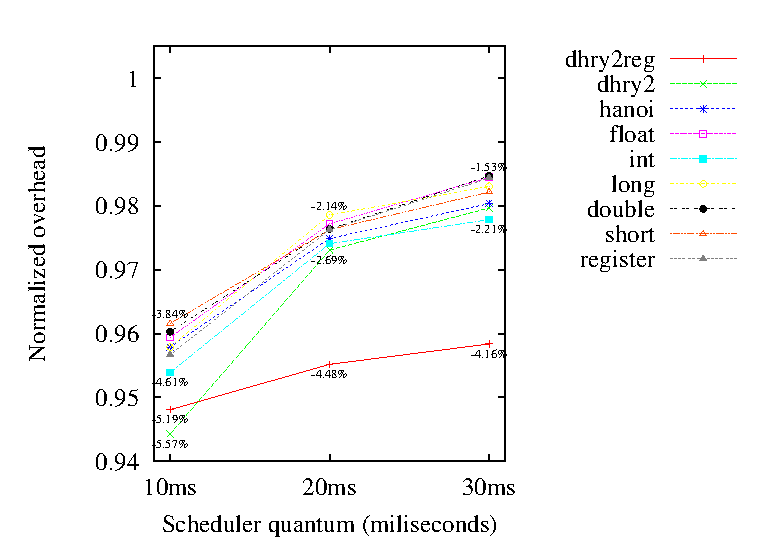
\includegraphics[width=0.6\textwidth]{chapter6/figures/bench_cpu}
	\caption{Performance overhead for user-land applications relative to non-virtualized performance.}
	\label{fig:bench_cpu}
\end{figure}

Each benchmark was performed 10,000 times to determine the average execution time. Figures \ref{fig:bench_cpu} and \ref{fig:bench_syscall} shows the normalized performance results for the user-land and syscall application groups. As expected, the overhead increased slightly with a smaller quantum due the increasing hypervisor intervention. In the user-land group, dhry2 was the most affected application with a performance penalty of 5.57\% when compared to a 10ms scheduler quantum. Additionally, most of the applications suffered an overhead of less than 3\% with a 30ms scheduler quantum. The syscall group suffered a greater performance impact since the benchmark force context-switching between the user and kernel-space in the Linux guest. In the worst case, the syscall close resulted in a penalty of 15.25\% performance loss with a 10ms scheduler quantum. However, for the majority of the cases the overhead was lower than 9\%. 

\begin{figure}[!hbtp]
	\centering
	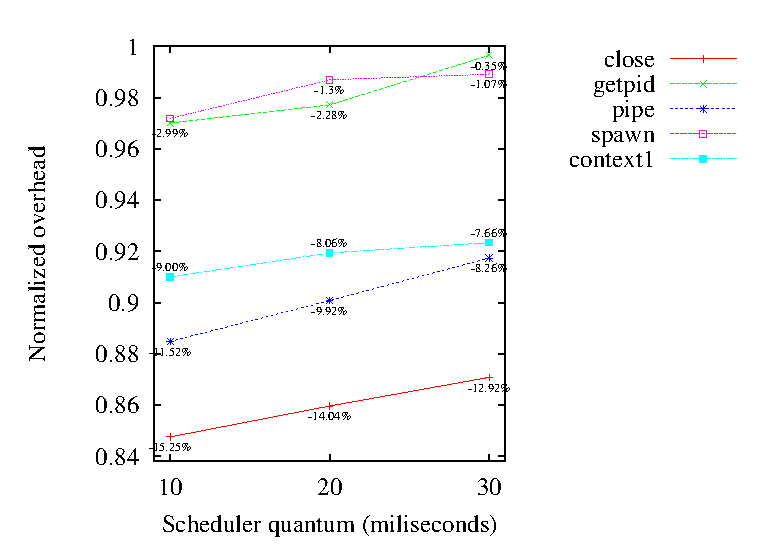
\includegraphics[width=0.6\textwidth]{chapter6/figures/bench_syscall}
	\caption{Performance overhead for syscall applications relative to non-virtualized performance.}
	\label{fig:bench_syscall}
\end{figure}


\subsection{IO-bound Benchmark}  

The Hellfire Hypervisor supports the SEAD-3's network device directly mapped to the Linux guest allowing it to receive network packages without any hypervisor intervention. The Iperf tool was used to measure the network bandwidth between the SEAD-3 board and a Linux host. Thus, it was possible to determine how our virtualization layer affects the I/O performance of the network device when directly mapped. Iperf consists of a client/server application originally developed by NLANR/DAST as a tool for measuring maximum TCP and UDP bandwidth performance \cite{iperf2004}. In this experiment, the Iperf server was executed on a Linux host and the Iperf client on the SEAD-3 board. Thus, the Iperf TCP bandwidth was measured for 1 minute for each experiment case. Figure \ref{fig:iperf} shows the results. The throughput was 8.32 Mbits/second for the native Linux execution. With a 30 ms scheduler quantum, the overhead was 1.84\%. As expected, the overhead increased slightly with a smaller quantum reaching 4.39\% for a 10 ms quantum. Even with smaller quanta, the overall results are optimistic and can be attributed to minimal hypervisor intervention. 

\begin{figure}[!hbtp]
	\centering
	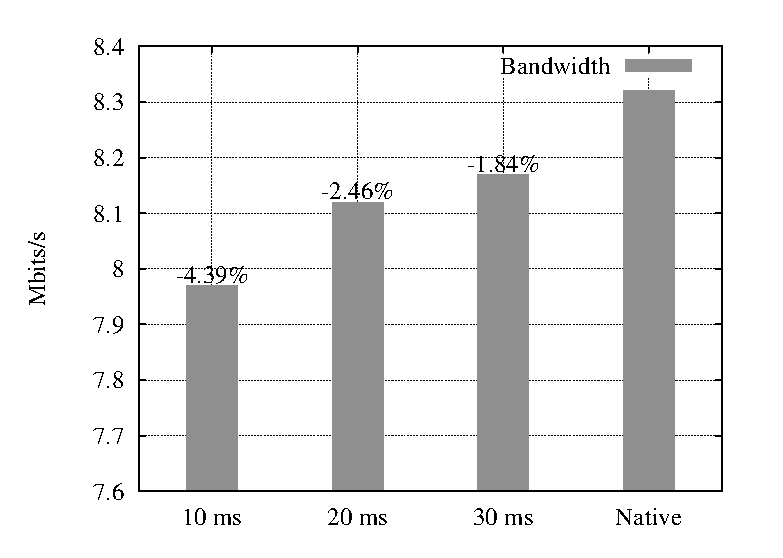
\includegraphics[width=0.6\textwidth]{chapter6/figures/iperf}
	\caption{Iperf bandwidth results for TCP protocol comparing native versus virtualized execution with different hypervisor's scheduler quantum.}
	\label{fig:iperf}
\end{figure}
    
\section{Overhead Impact on HellfireOS} 
\label{section:hellfireOverhead}

This section evaluates the virtualization overhead imposed to the Hellfire OS. The HellfireOS's kernel executes only in kernel mode. Thus, it does not perform memory isolation between tasks because it does not implement memory management. However, the HellfireOS can execute on small processors without MMU support. Two different benchmarks were ported to the RTOS for evaluation purposes. The first algorithm was the adaptive differential pulse-code modulation (ADPCM)  \cite{cummiskey1973}. ADPCM is a technique to convert analog sound to binary information. It is used for voice communication and sound storage. The second was a data compression algorithm, where only compression is done in a buffer containing totally random data. The implementation of this algorithms was obtained from the WCET Project\footnote{http://www.mrtc.mdh.se/projects/wcet/benchmarks.html}, which keeps a large number of benchmark programs. Thus, the source-code was ported to the HellfireOS' APIs.

\begin{figure}[!hbtp]
	\centering
	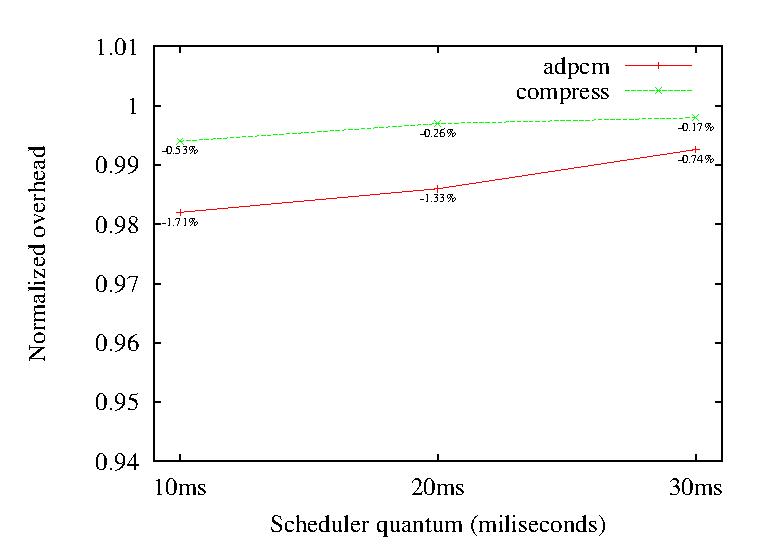
\includegraphics[width=0.6\textwidth]{chapter6/figures/bench_cpu_hell}
	\caption{Performance overhead for CPU intensive applications relative to non-virtualized performance.}
	\label{fig:bench_cpu_hell}
\end{figure}

Both algorithms were performed natively and virtualized with hypervisor scheduler's quantum of 10, 20 and 30ms. The average time for 10,000 executions for each algorithm was obtained. Figure \ref{fig:bench_cpu_hell} shows the normalized results relative to non-virtualized execution. The worst case overhead was 1.71\% for the ADPCM algorithm executing with a scheduler quantum of 10ms. The measured overhead is still smaller than the overhead for Linux CPU-Bound applications (see Figure \ref{fig:bench_cpu}). Despite the HellfireOS to be a lightweight RTOS requiring fewer computation resources, the set of processor resources saved during context-switching is the same of the Linux. A possible explanation for the lower overhead in the HellfireOS is cache effects since the code size impact over the processor's cache was not considered in this study. Linux has a larger code size than HellfireOS what can make it more susceptible to cache effects when submitted to hypervisor interventions. However, more research is necessary to determine the exact cause of the smaller overhead in the HellfireOS benchmarks. 



\section{Interrupt Delivery Delay}
\label{section6:interruption-delay}

This experiment was performed to test the effectiveness of the fast interrupt delivery mechanism as described in Section \ref{section5:interrupt}. Thus, the following experiments show how the response delay of the OS's interrupt handler is affected by the hypervisor interference and how the proposed solution can improve overall system responsiveness. The virtualized system setup consisted of a Linux guest with a variable number of concurrent VMs executing HellfireOS instances. The Ethernet device was directly mapped to the Linux guest. For interrupt delay measurement, the Internet Control Message Protocol (ICMP) was used to send echo request messages from an Intel Xeon server running Debian Linux 7.8 directly connected to the SEAD-3 board. For all test cases, ICMP messages were sent at intervals of 50 milliseconds (20Hz) using the Linux ping application\footnote{http://linux.die.net/man/8/ping}. Each test case consisted of 10,000 echo request messages followed by their respective response messages (echo reply). Thus, the round-trip time (RTT) \cite{tanenbaum2011} of the messages for network communication with the SEAD-3 board was determined. Delays in the Linux interrupt handler caused by the hypervisor impacting directly in the RTT were expected. Finally, the average delay ($\overline{x}$), standard deviation ($s$), median ($m$) and the $95^{th}$ percentile ($p^{th}$) for the RTT of the messages were determined. Results for the Linux/MIPS native (non-virtualized) execution can be viewed in Table \ref{table:delaylinux}. Table \ref{table:delay} shows the results of all experiments performed using virtualization. Lines three and five depict the behavior of the recycled quantum and reset quantum policies with half of the VMs marked as non-preemptable. Figure \ref{fig:native} shows the corresponding histogram for the RTT of native Linux execution messages. The data sets used to generate the results of the lines 1 to 5 of the Table \ref{table:delay} are represented in the histograms of the Figures \ref{fig:non-policy}, \ref{fig:fast-recycling}, \ref{fig:fast-reset}, \ref{fig:fast-recycling-preempt} and \ref{fig:fast-reset-preempt}.

%Figures \ref{fig:histogram_2vm}, \ref{fig:histogram_4vm} and \ref{fig:histogram_6vm} depict the histogram for the RTT of the messages  for 2, 4 and 6 VMs.

\begin{sidewaystable}[!hbtp]
\centering
\caption{Average ($\overline{x}$), standard deviation ($s$), median ($m$) and $95^{th}$ percentile ($p^{th}$) for RTT of the messages in milliseconds for Linux native execution.}
\label{table:delaylinux}
\begin{tabular}{lllll}
\hline \hline
\multicolumn{1}{c}{\textbf{Strategy}} & \multicolumn{1}{c}{\textbf{$\overline{x}$}} & \multicolumn{1}{c}{\textbf{$s$}} & \multicolumn{1}{c}{\textbf{$m$}} & \multicolumn{1}{c}{\textbf{$p^{th}$}} \\ \hline
\textbf{Linux interrupt police}       & 1.073                          & 0.107                          & 1.05                           & 1.24                           \\ \hline
\end{tabular}
\vspace{2\baselineskip}
\caption{Average ($\overline{x}$), standard deviation ($s$), median ($m$) and $95^{th}$ percentile ($p^{th}$) for RTT of the messages in milliseconds for virtualized Linux execution.}
\label{table:delay}
\begin{tabular}{llllllllllllll}
\hline \hline
\multirow{2}{*}{\textbf{\#}} & \multicolumn{1}{c}{\multirow{2}{*}{\textbf{Strategy}}} & \multicolumn{4}{c}{\textbf{2 VMs}}                & \multicolumn{4}{c}{\textbf{4 VMs}}                & \multicolumn{4}{c}{\textbf{6 VMs}}                \\ \cline{3-14} 
                             & \multicolumn{1}{c}{}                                   & \textbf{$\overline{x}$} & \textbf{$s$} & \textbf{$m$} & \textbf{$p^{th}$} & \textbf{$\overline{x}$} & \textbf{$s$} & \textbf{$m$} & \textbf{$p^{th}$} & \textbf{$\overline{x}$} & \textbf{$s$} & \textbf{$m$} & \textbf{$p^{th}$} \\ \hline
\textbf{1}                   & \textbf{Without interrupt police}                      & 9.35       & 10.21      & 2.73       & 29.5       & 30.7       & 29.6       & 86.4       & 66.29      & 66.29      & 49.40      & 66.90      & 145        \\
\textbf{2}                   & \textbf{Recycled quantum (R.Q.)}                      & 1.87       & 4.09       & 1.2        & 1.83       & 12.05      & 1.56       & 5.52       & 6.90       & 6.90       & 21.04      & 1.44       & 50.4       \\
\textbf{3}                   & \textbf{R.Q. with non-preempt. VCPU}                   & 9.28       & 10.16      & 2.70       & 29.1       & 12.90      & 1.66       & 29.1       & 9.72       & 9.72       & 19.83      & 1.68       & 31.5       \\
\textbf{4}                   & \textbf{Reset quantum (Res.Q.)}                        & 1.29       & 0.81       & 1.11       & 1.69       & 2.49       & 1.55       & 1.85       & 2.50       & 2.50       & 10.39      & 1.22       & 1.82       \\
\textbf{5}                   & \textbf{Res.Q. with non-preempt. VCPU}                 & 2.86       & 3.17       & 1.1        & 9.89       & 8.61       & 8.19       & 2.07       & 21.1       & 10.49      & 12.32      & 1.71       & 30.7       \\ \hline
\end{tabular}
\end{sidewaystable}


\begin{figure}[!hbtp]
	\centering
	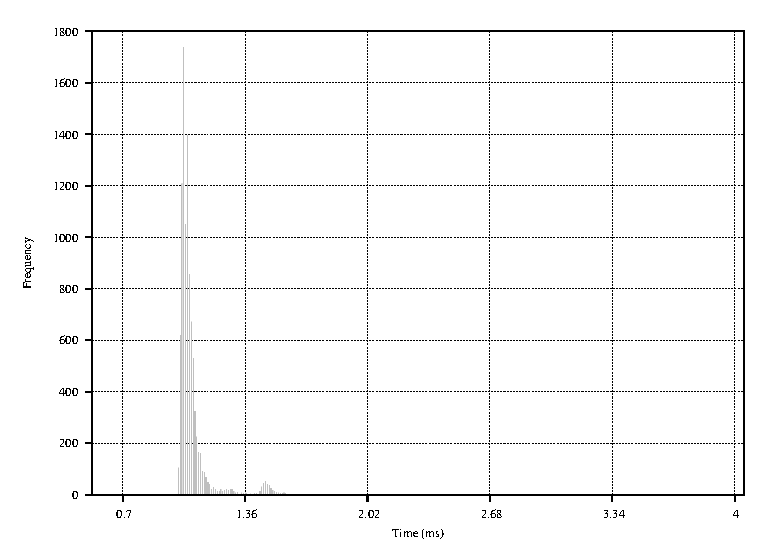
\includegraphics[width=0.45\textwidth]{chapter6/figures/ping_native}
	\caption{Histogram for RTT of the messages for native execution of the Linux/MIPS.}
	\label{fig:native}
\end{figure}

Once the native response time was obtained, the results were compared to virtualized instances of the Linux/MIPS. For each test case, the guest Linux/MIPS shared the processor with VCPUs in different system configurations: 2 VMs (one Linux/MIPS and one BE-VCPU), 4 VMs (one Linux/MIPS and three BE-VCPUs) and 6 VMs (one Linux/MIPS and five BE-VCPUs). Each BE-VCPU was performing the HellfireOS as a guest during the tests. For each configuration, tests were performed without any specific policy, consequently increasing the response delay. Line one of the Table \ref{table:delay} shows that the delay growth is proportional to the increasing number of concurrent VMs. Figures \ref{fig:2vm}, \ref{fig:4vm} and \ref{fig:6vm} show the corresponding histogram to the RTT of the messages to the configuration of 2, 4 and 6 VMs, respectively. Observe the increased horizontal scale of the histogram in the figures. These results show that the hypervisor significantly affected the response time when compared to native results. This was expected since the VMs were scheduled in a round-robin algorithm, and an interrupt on the Ethernet device must wait for the next Linux/MIPS execution. Moreover, the hypervisor scheduler time quantum is 30 milliseconds. For example, in a system configuration of 4 VMs the delay to handle an interrupt can be up to 90 milliseconds if the guest Linux/MIPS is the last in the round-robin queue. 

\begin{figure}[!hbtp]
\centering
\subfigure[Two VMs.]{
    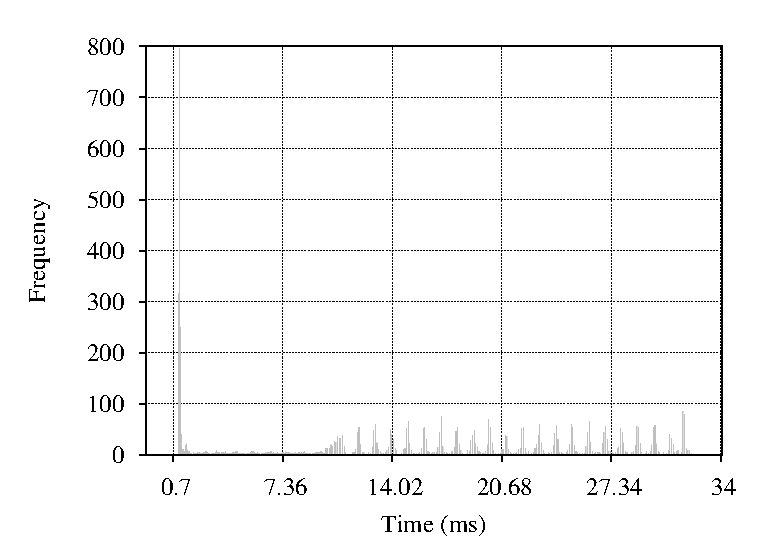
\includegraphics[width=.315\textwidth]{chapter6/figures/2VM}
    \label{fig:2vm}
}
\subfigure[Four VMs.]{
    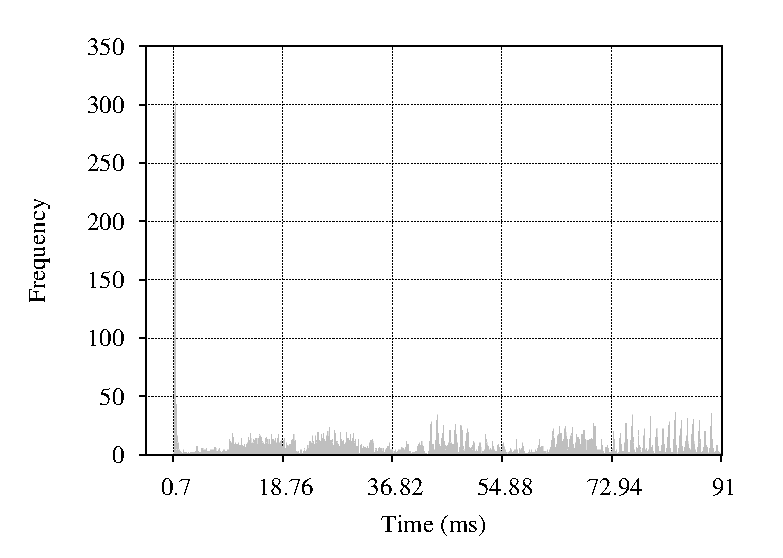
\includegraphics[width=.315\textwidth]{chapter6/figures/4VM}
    \label{fig:4vm}
}
\subfigure[Six VMs.]{
    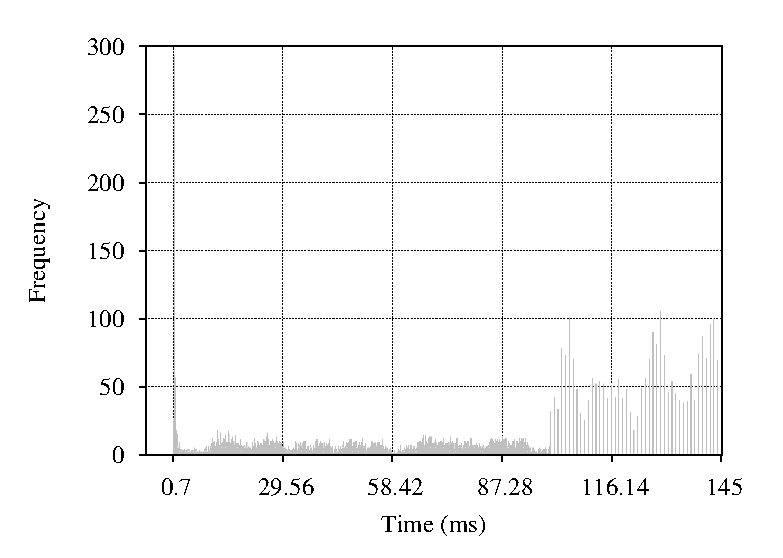
\includegraphics[width=.315\textwidth]{chapter6/figures/6VM}
    \label{fig:6vm}
}
\captionsetup{justification=centering}
\caption{Histogram for RTT of the messages without policy.}
\label{fig:non-policy}
\end{figure}

\begin{figure}[!hbtp]
\centering
\subfigure[Two VMs.]{
    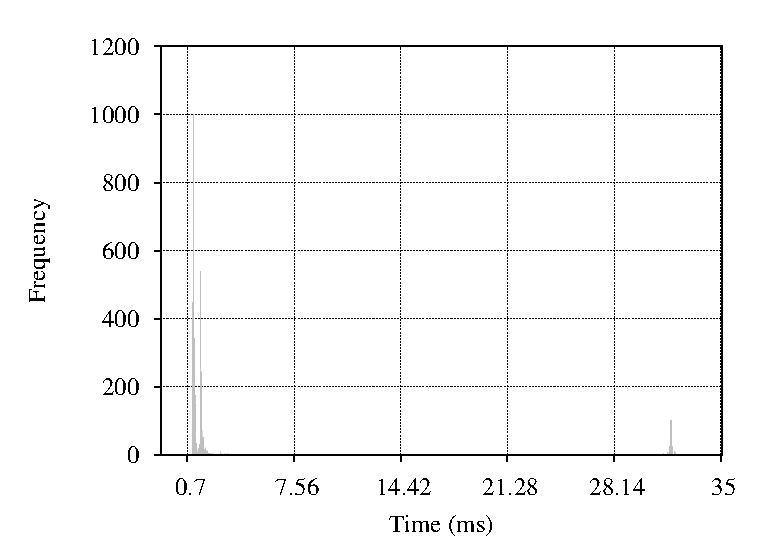
\includegraphics[width=.315\textwidth]{chapter6/figures/2VM-fast-same}
    \label{fig:2vm-fast-same}
}
\subfigure[Four VMs.]{
    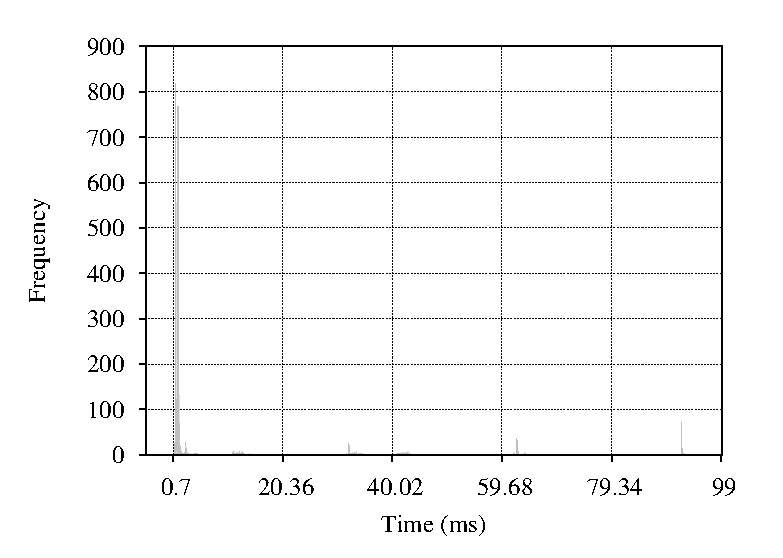
\includegraphics[width=.315\textwidth]{chapter6/figures/4VM-fast-same}
    \label{fig:4vm-fast-same}
}
\subfigure[Six VMs.]{
    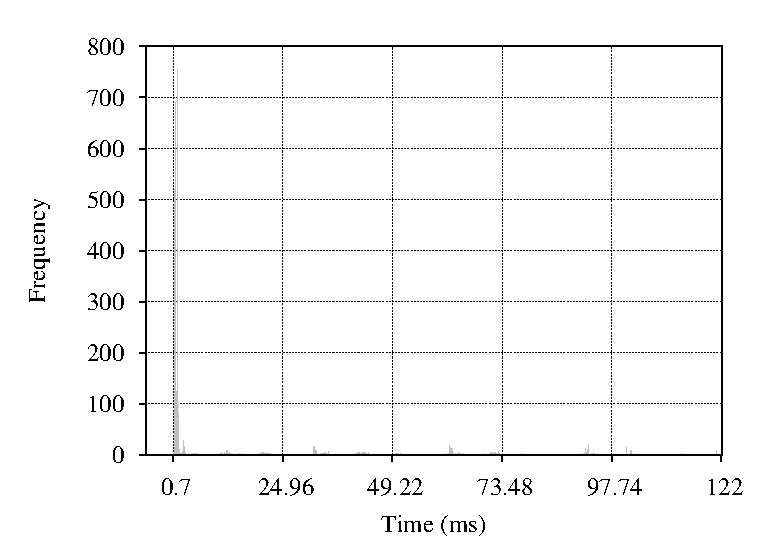
\includegraphics[width=.315\textwidth]{chapter6/figures/6VM-fast-same}
    \label{fig:6vm-fast-same}
}
\captionsetup{justification=centering}
\caption{Histogram for RTT of the messages with fast interrupt policy and quantum recycling.}
\label{fig:fast-recycling}
\end{figure}


%\begin{figure}[!hbtp]
%\centering
%\subfigure[Without policy.]{
%    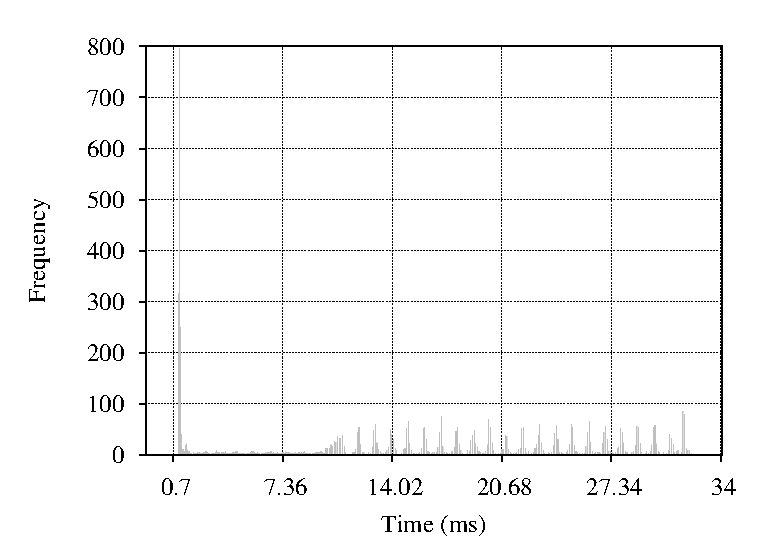
\includegraphics[width=.45\textwidth]{chapter6/figures/2VM}
%    \label{fig:2vm}
%}
%\subfigure[Fast interrupt policy and quantum recycling.]{
%    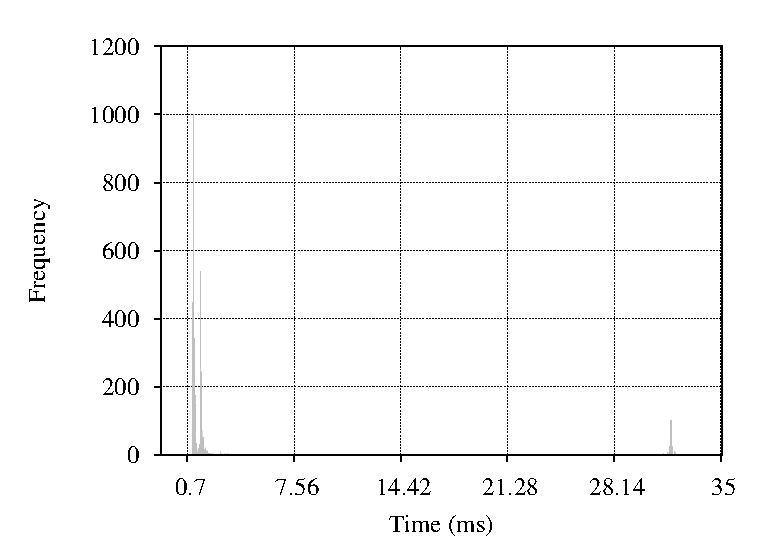
\includegraphics[width=.45\textwidth]{chapter6/figures/2VM-fast-same}
%    \label{fig:2vm-fast-same}
%}

%\subfigure[Fast interrupt policy and quantum reset.]{
%    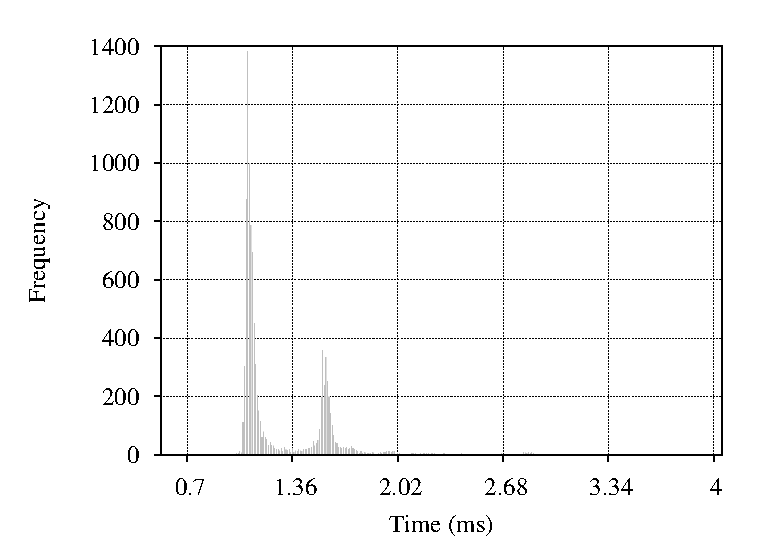
\includegraphics[width=.45\textwidth]{chapter6/figures/2VM-fast-new}
%    \label{fig:2vm-fast-new}
%}
%\subfigure[Fast interrupt policy and quantum reset with two non-preemptable VCPUs.]{
%    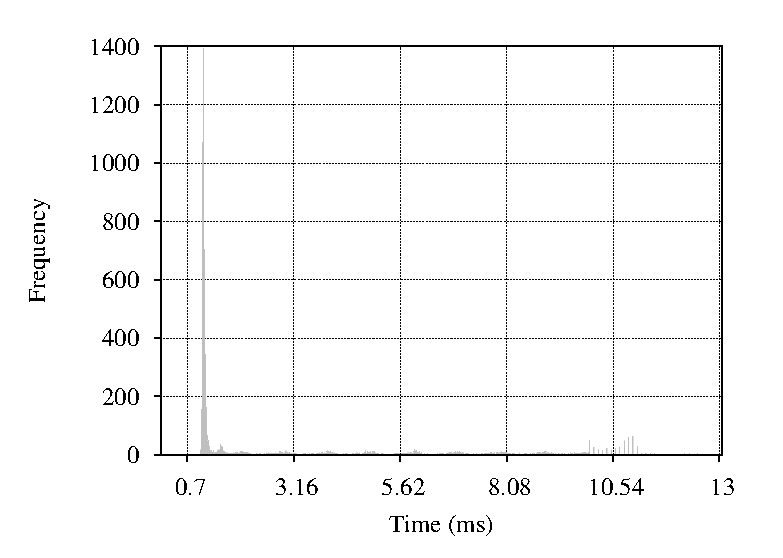
\includegraphics[width=.45\textwidth]{chapter6/figures/2VM-fast-new-1RTOS}
%    \label{fig:2vm-fast-new-rtos}
%}

%\subfigure[Fast interrupt policy and quantum recycling with two non-preemptable VCPUs.]{
%    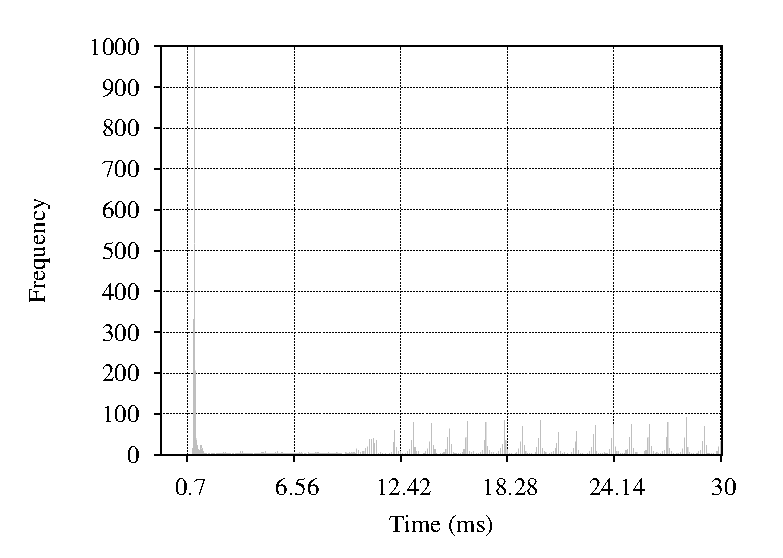
\includegraphics[width=.45\textwidth]{chapter6/figures/2VM-fast-same-1RTOS}
%    \label{fig:2vm-fast-same-rtos}
%}
%\captionsetup{justification=centering}
%\caption{Histogram for messages' RTT for a system configuration of 2 VCPUs.}
%\label{fig:histogram_2vm}
%\end{figure}

%\begin{figure}[!hbtp]
%\centering
%\subfigure[Without policy.]{
%    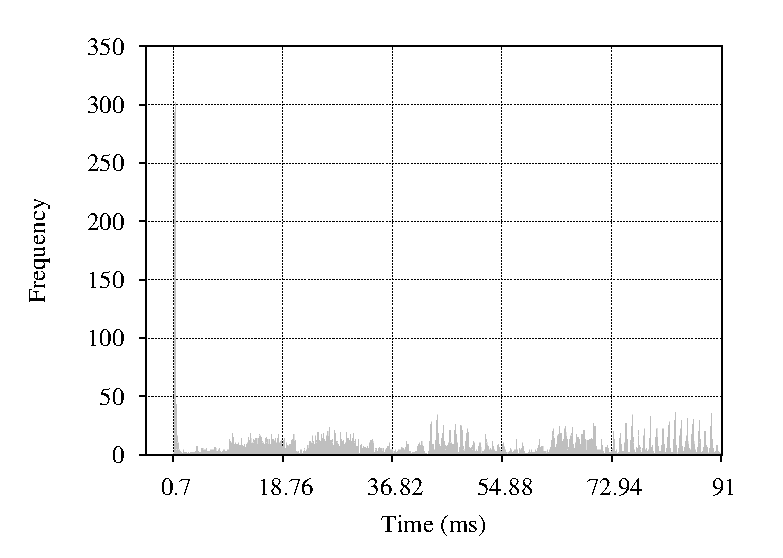
\includegraphics[width=.45\textwidth]{chapter6/figures/4VM}
%    \label{fig:4vm}
%}
%\subfigure[Fast interrupt policy and quantum recycling.]{
%    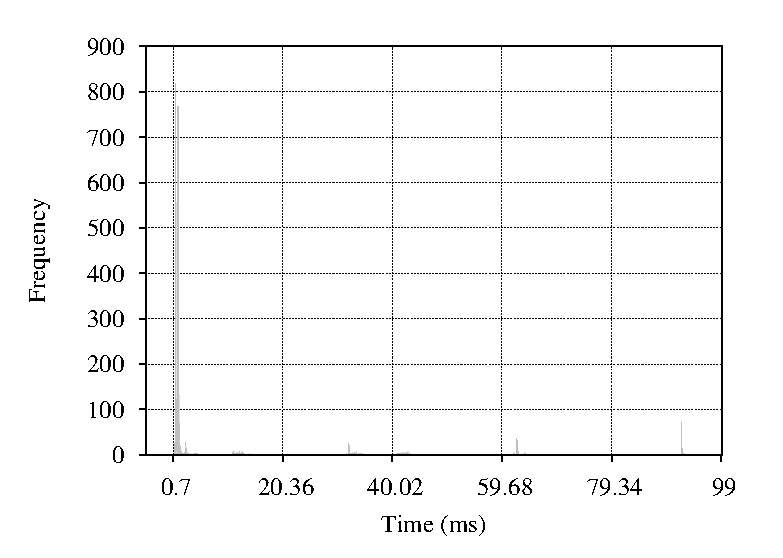
\includegraphics[width=.45\textwidth]{chapter6/figures/4VM-fast-same}
%    \label{fig:4vm-fast-same}
%}

%\subfigure[Fast interrupt policy and quantum reset.]{
%    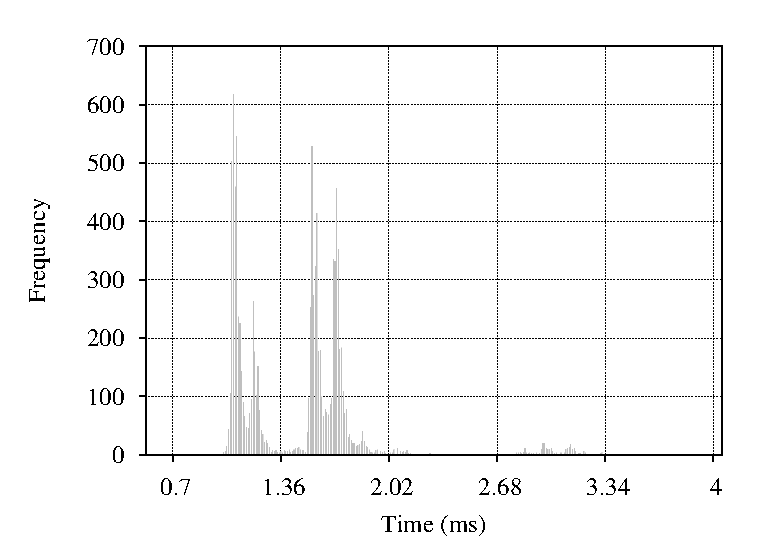
\includegraphics[width=.45\textwidth]{chapter6/figures/4VM-fast-new}
%    \label{fig:4vm-fast-new}
%}
%\subfigure[4 VMs with fast interrupt policy and quantum reset with two non-preemptable VCPUs.]{
%    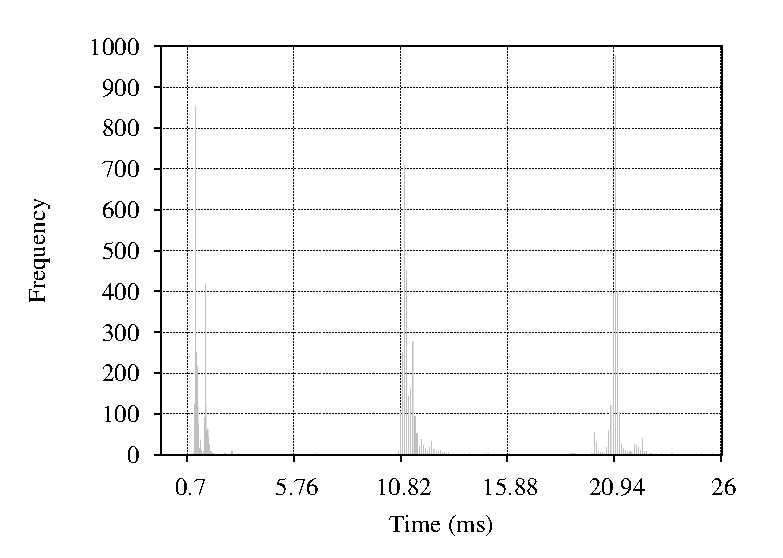
\includegraphics[width=.45\textwidth]{chapter6/figures/4VM-fast-new-2RTOS}
%    \label{fig:4vm-fast-new-rtos}
%}

%\subfigure[4 VMs with fast interrupt policy and quantum recyling with two non-preemptable VCPUs.]{
%    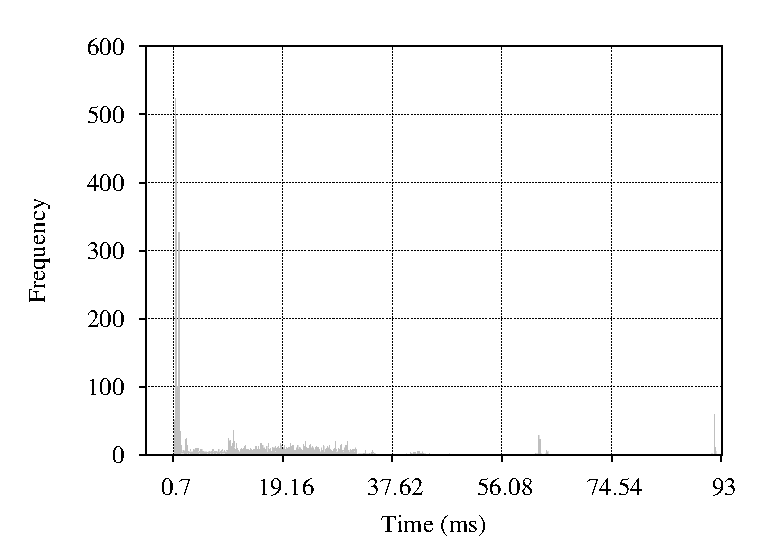
\includegraphics[width=.45\textwidth]{chapter6/figures/4VM-fast-same-2RTOS}
%    \label{fig:4vm-fast-same-rtos}
%}
%\captionsetup{justification=centering}
%\caption{Histogram for messages' RTT for a system configuration of 4 VCPUs.}
%\label{fig:histogram_4vm}
%\end{figure}

After determining how the hypervisor affects the interrupt response time, two different policies were tested to discover which one gives the best approximation to the native response time. Line two of Table \ref{table:delay} (Recycled quantum) shows the results when applied the fast interrupt policy together with the recycled quantum scheme (as explained in Figure \ref{subfig:interruptdelayB}). This technique improves the overall results. However, the recycled quantum mechanism has a drawback. If the remaining of quantum time is not sufficient to finish the interrupt handler routine, it will be finished only in the next guest's execution. Figures \ref{fig:2vm-fast-same}, \ref{fig:4vm-fast-same} and \ref{fig:6vm-fast-same} depict the corresponding histogram of the RTT of the messages for the configuration of 2, 4 and 6 VMs, respectively. Most interrupts have a fast response as shown by the peak near 0.7 milliseconds. For such cases, the interrupt assertion happened during the guest execution or the remaining quantum time was enough for the interrupt handler to finish its job. However, some messages experience a long delay and the response time is close to  multiples of 30 milliseconds. Thus, the remaining quantum time was not enough and the interrupt handler only finished in the next execution. 

\begin{figure}[!hbtp]
\centering
\subfigure[Two VMs.]{
    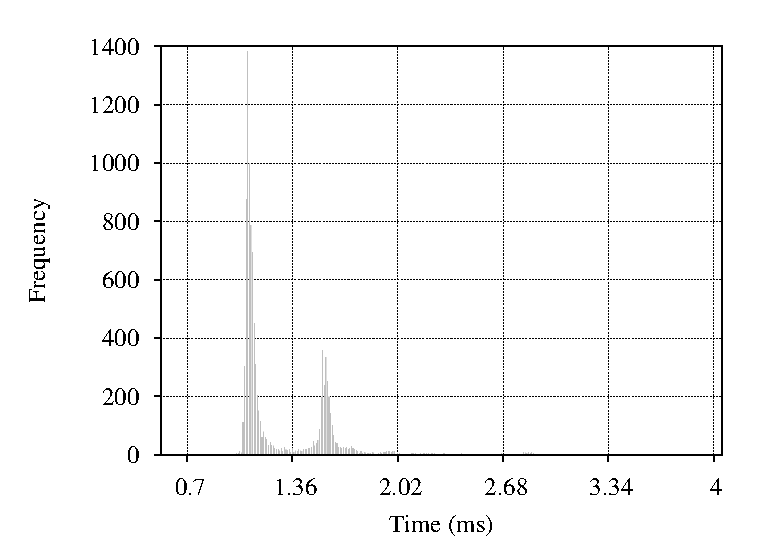
\includegraphics[width=.315\textwidth]{chapter6/figures/2VM-fast-new}
    \label{fig:2vm-fast-new}
}
\subfigure[Four VMs.]{
    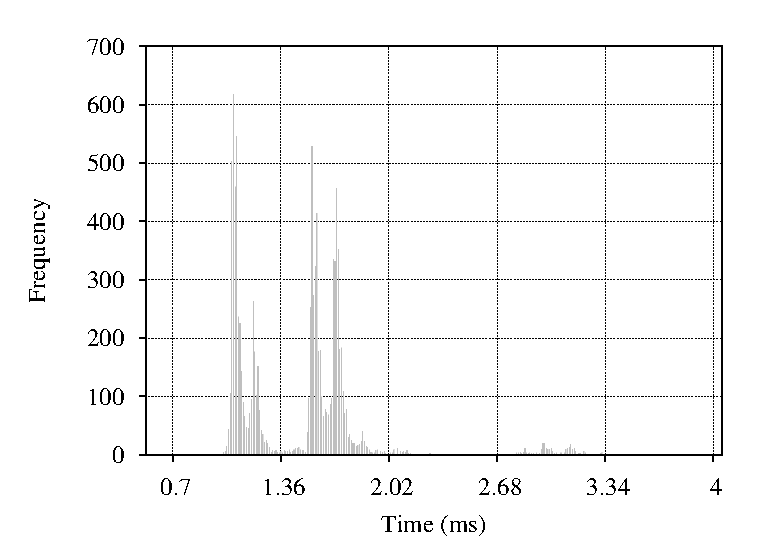
\includegraphics[width=.315\textwidth]{chapter6/figures/4VM-fast-new}
    \label{fig:4vm-fast-new}
}
\subfigure[Six VMs.]{
    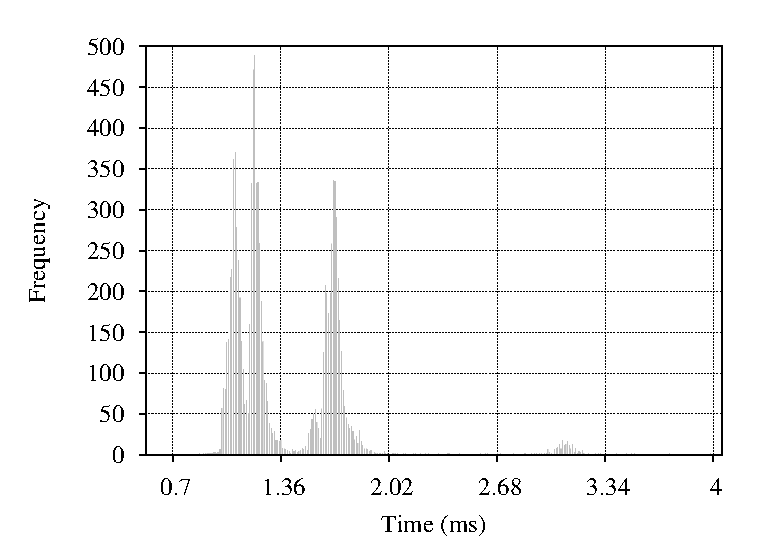
\includegraphics[width=.315\textwidth]{chapter6/figures/6VM-fast-new}
    \label{fig:6vm-fast-new}
}
\captionsetup{justification=centering}
\caption{Histogram for RTT of the messages with fast interrupt policy and quantum reset.}
\label{fig:fast-reset}
\end{figure}


Line four of Table \ref{table:delay} (Reset quantum) shows the results of the fast interrupt policy with a reset quantum scheme. For 2 VM configurations, the average and standard deviation delays are close to native execution. In the 4 and 6 VM system configurations, the results are slightly higher but better than results for the recycled quantum scheme. Figures \ref{fig:2vm-fast-new}, \ref{fig:4vm-fast-new} and \ref{fig:6vm-fast-new} show the corresponding histogram of the RTT of the messages for the configuration of 2, 4 and 6 VMs, respectively. Observe that the horizontal scale in the figure is similar to native execution. These histograms show two peaks. The peak for delays  under one millisecond represents interrupt assertions that happened when the target guest OS was executing. The second peak for delays greater than one millisecond represents interrupt assertions that caused a context switch because the target guest was not executing. 

\begin{figure}[!hbtp]
\centering
\subfigure[Two VMs, one non-preempt.]{
    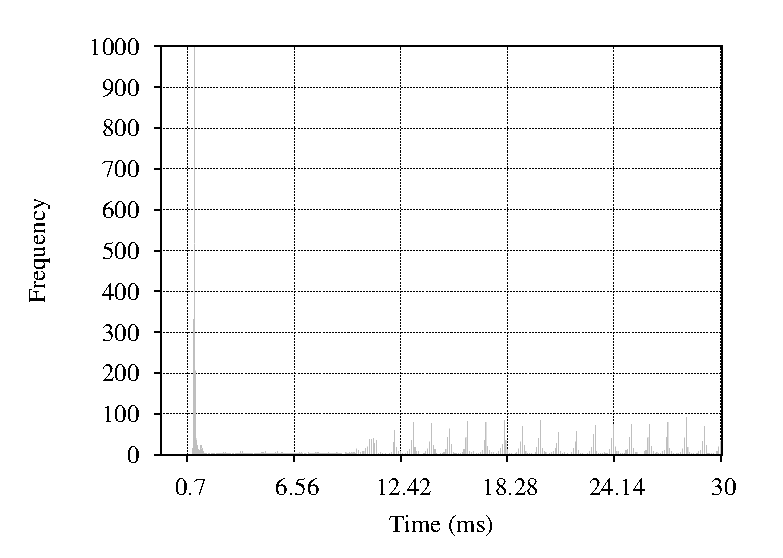
\includegraphics[width=.315\textwidth]{chapter6/figures/2VM-fast-same-1RTOS}
    \label{fig:2vm-fast-same-rtos}
}
\subfigure[Four VMs, two non-preempt.]{
    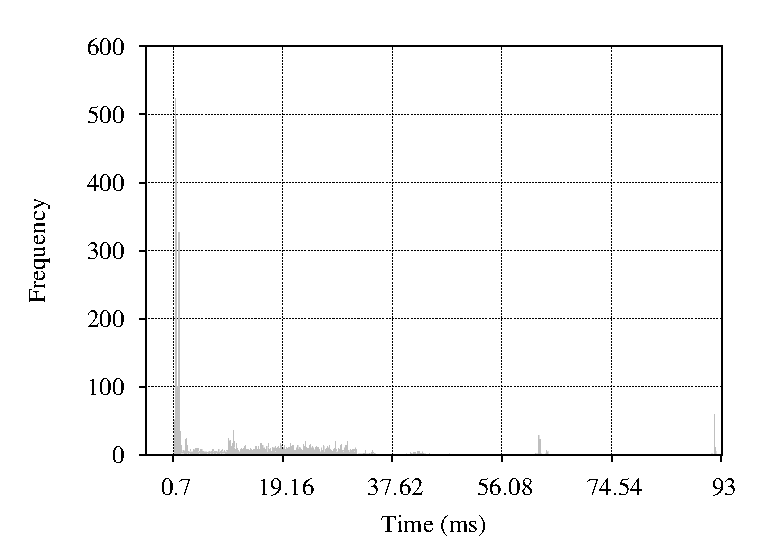
\includegraphics[width=.315\textwidth]{chapter6/figures/4VM-fast-same-2RTOS}
    \label{fig:4vm-fast-same-rtos}
}
\subfigure[Six VMs, three non-preempt.]{
    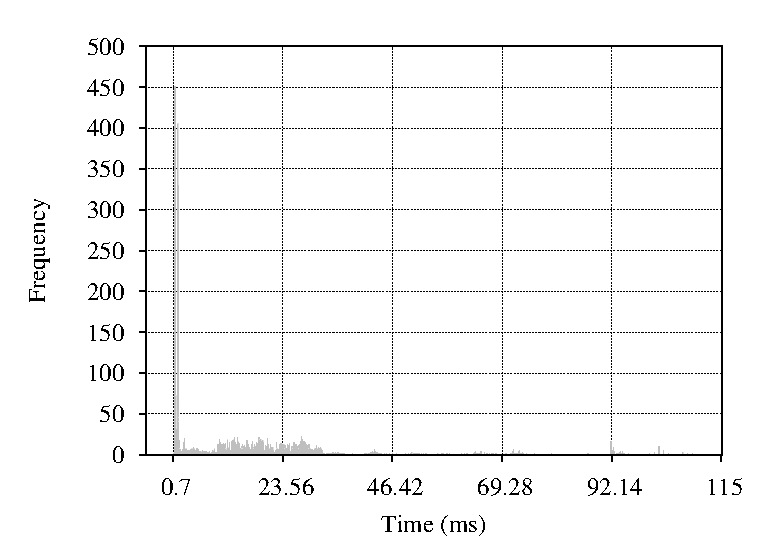
\includegraphics[width=.315\textwidth]{chapter6/figures/6VM-fast-same-3RTOS}
    \label{fig:6vm-fast-same-rtos}
}
\captionsetup{justification=centering}
\caption{Histogram for RTT of the messages with fast interrupt policy and quantum recycling with non-preemptable VCPUs.}
\label{fig:fast-recycling-preempt}
\end{figure}

Finally, lines 3 (R.Q. with non-preempt. RTOS) and 5 (Res.Q. with non-preempt. RTOS) of Table \ref{table:delay} show the results for recycled quantum and reset quantum schemes in the presence of non-preemptive guests. For each configuration, half of the guests were marked as non-preemptive. The presence of non-preemptive guests increased the average and standard deviation delays, but the results are better than the approach without any interrupt policy. Figures \ref{fig:4vm-fast-same-rtos}, \ref{fig:6vm-fast-same-rtos} and \ref{fig:6vm-fast-same-rtos} show the histograms for recycled quantum with non-preemptive guests for 2, 4 and 6 VMs. Figures \ref{fig:4vm-fast-new-rtos}, \ref{fig:6vm-fast-new-rtos} and \ref{fig:6vm-fast-new-rtos} show the histograms for reset quantum with non-preemptive guests for 2, 4 and 6 VMs. 

\begin{figure}[!hbtp]
\centering
\subfigure[Two VMs, one non-preempt.]{
    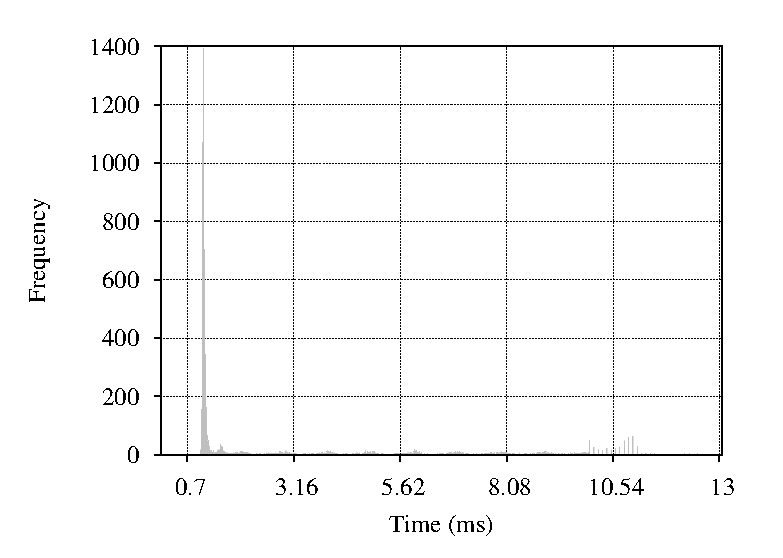
\includegraphics[width=.315\textwidth]{chapter6/figures/2VM-fast-new-1RTOS}
    \label{fig:2vm-fast-new-rtos}
}
\subfigure[Four VMs, two non-preempt.]{
    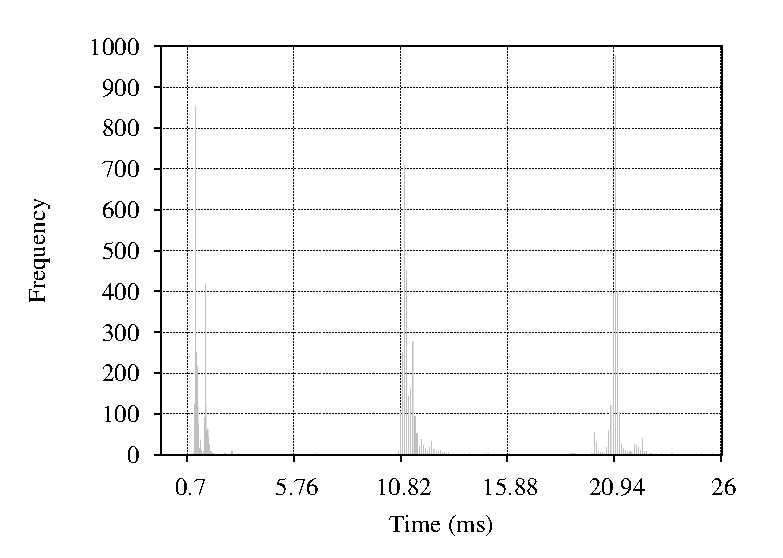
\includegraphics[width=.315\textwidth]{chapter6/figures/4VM-fast-new-2RTOS}
    \label{fig:4vm-fast-new-rtos}
}
\subfigure[Six VMs, three non-preempt.]{
    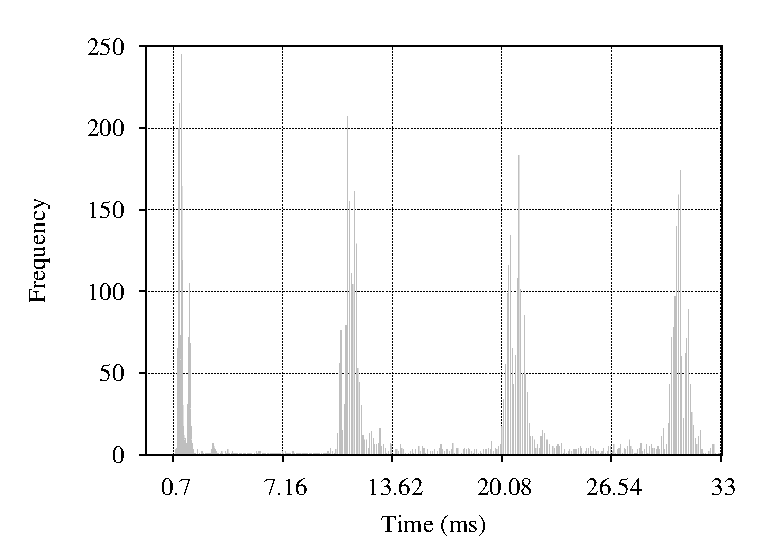
\includegraphics[width=.315\textwidth]{chapter6/figures/6VM-fast-new-3RTOS}
    \label{fig:6vm-fast-new-rtos}
}
\captionsetup{justification=centering}
\caption{Histogram for RTT of the messages with fast interrupt policy and quantum reset with non-preemptable VMs.}
\label{fig:fast-reset-preempt}
\end{figure}

%\begin{figure}[!hbtp]
%\centering
%\subfigure[Without policy.]{
%    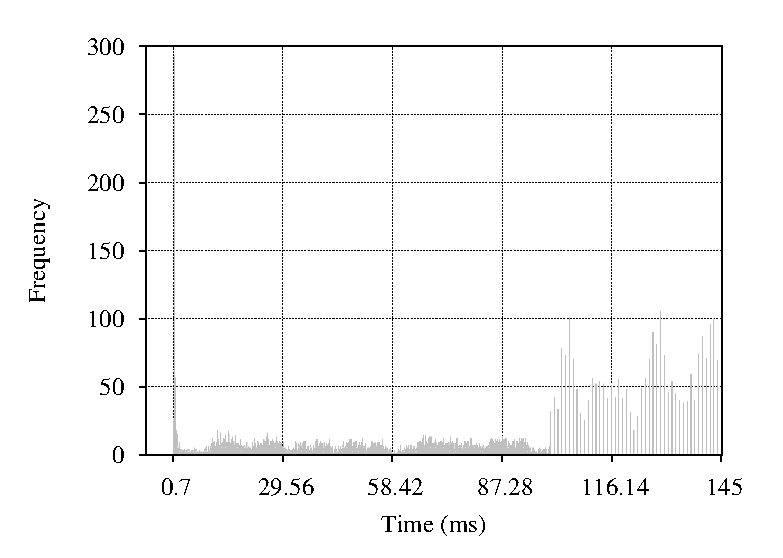
\includegraphics[width=.45\textwidth]{chapter6/figures/6VM}
%    \label{fig:6vm}
%}
%\subfigure[Fast interrupt policy and quantum recycling.]{
%    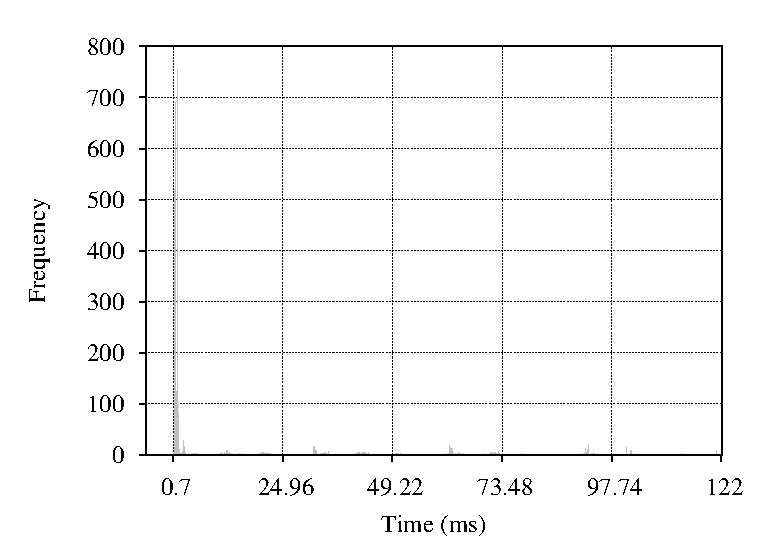
\includegraphics[width=.45\textwidth]{chapter6/figures/6VM-fast-same}
%    \label{fig:6vm-fast-same}
%}

%\subfigure[Fast interrupt policy and quantum reset.]{
%    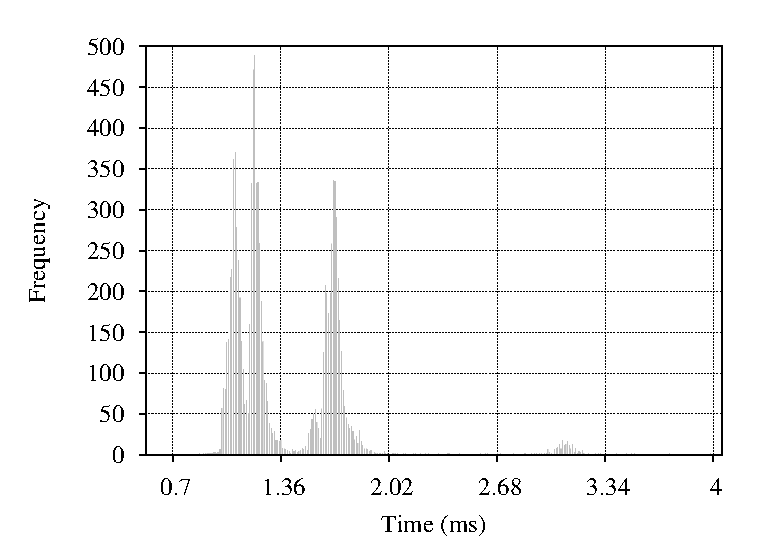
\includegraphics[width=.45\textwidth]{chapter6/figures/6VM-fast-new}
%    \label{fig:6vm-fast-new}
%}
%\subfigure[Fast interrupt policy and quantum reset with three non-preemptable VCPUs.]{
%    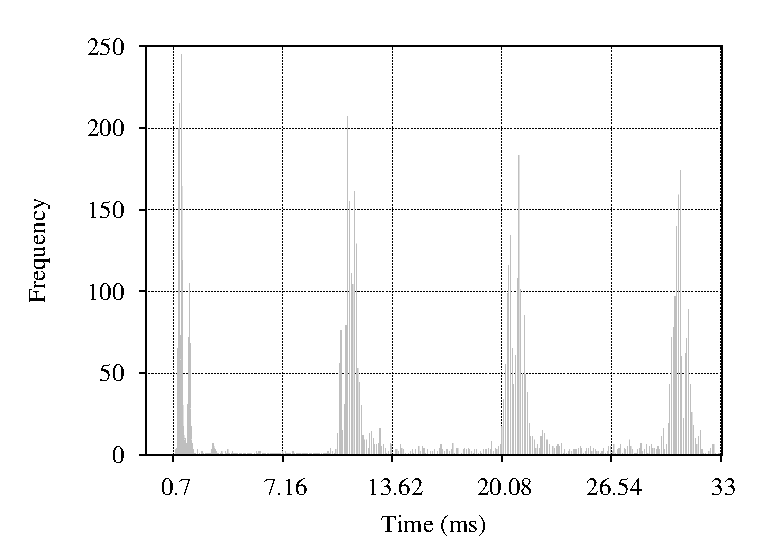
\includegraphics[width=.45\textwidth]{chapter6/figures/6VM-fast-new-3RTOS}
%    \label{fig:6vm-fast-new-rtos}
%}

%\subfigure[Fast interrupt policy and quantum reset with three non-preemptable VCPUs.]{
%    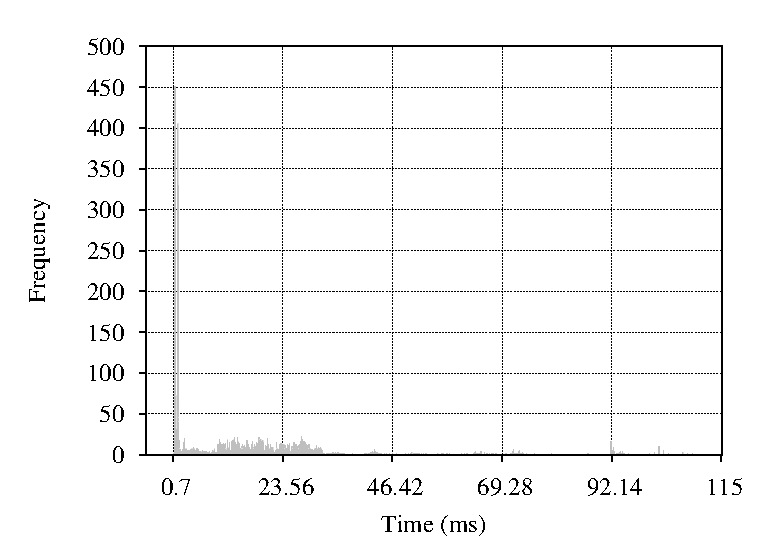
\includegraphics[width=.45\textwidth]{chapter6/figures/6VM-fast-same-3RTOS}
%    \label{fig:6vm-fast-same-rtos}
%}

%\captionsetup{justification=centering}
%\caption{Histogram for messages' RTT for a system configuration of 6 VCPUs.}
%\label{fig:histogram_6vm}
%\end{figure}

The reset quantum scheme associated with the fast interrupt policy presented better results than the recycled quantum. However, this scheme may be disruptive for RTOSs with strict timing constraints and can not be combined with the EDF scheduler algorithm. The EDF implemented computes the next time slot execution of the RT-VCPUs based on the number of quanta performed. The reset quantum scheme breaks the correspondence between time and the completed number of quanta. The recycle quantum mechanism keeps a substantial time isolation between guests. Thus, it must be used when predictability is more important than low response time. Additionally, the fast interrupt policy allows for the reduction of hypervisor interference for  values close to  non-virtualized systems in certain configurations. Finally, the proposed mechanism is flexible and allows for customization of the hypervisor for specific applications for any number of guest OSs. Section \ref{subsection:int_rtvcpus} describes a scenario where the fast interrupt delivery policy is combined with RT-VCPUs.


\section{Inter-VM Communication Response Time}
\label{subsection:intervm}

In order to calculate the RTT of the messages to the inter-VM communication mechanism, it was implemented an echo server application, which replayed all messages received, in the HellfireOS. A client application was implemented in the Linux to send 16, 32 and 64 byte messages after reading the server's response. The measurement of the average RTT for 10,000 messages for each different size resulted in 59.90, 59.90 and 59.99ms with a standard deviation of 0.71ms, 0.71ms and 0.69ms, respectively. An increase in the message size from 16 to 64 bytes did not significantly impact the RTT. The imposed overhead was caused by message copies from the sender's buffer to the target VCPU and to the receiver's buffer. The message exchange mechanism caused an additional copy but allowed  the hypervisor to have better communication control,  similar to pipes in Linux. Figure \ref{fig:intervm} depicts the histogram of the RTT's distribution for 16, 32 and 64 byte messages. In this experiment, we applied our fast interrupt delivery policy. Thus, once the Linux guest sent a message, the hypervisor rescheduled the VMs to the target guest resulting in a faster response and reducing the standard deviation.

\begin{figure}[!hbtp]
	\centering
	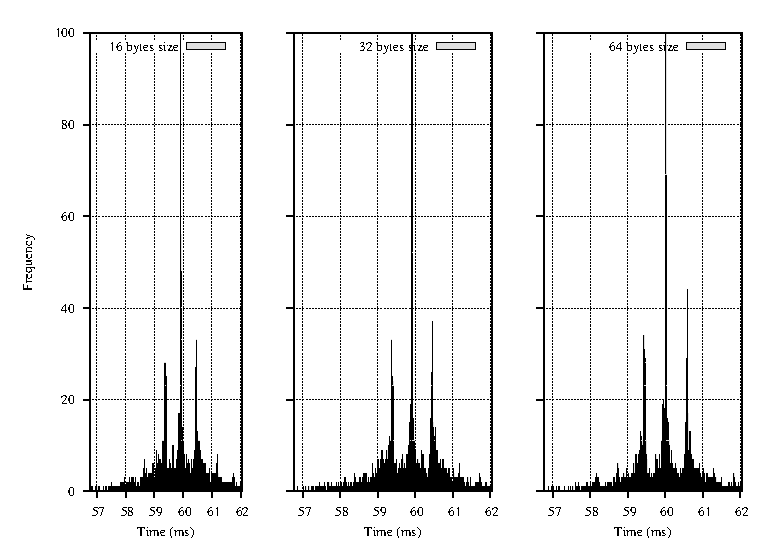
\includegraphics[width=0.50\textwidth]{chapter6/figures/intermv-jitter-3}
	\caption{RTT's histograms for inter-VM communication using the Hellfire Hypervisor communication mechanism.}
	\label{fig:intervm}
\end{figure}


\section{Real-time Services Performance}
\label{section6:realtimeservices}

This section depicts experiments related to real-time services. Thus, RT-VMs are used to provide tasks performed by RT-VCPUs. Subsection \ref{subsection:rtdelay} describes an experiment to determine the real-time scheduler delay caused by the EDF implementation in a system with an increasing number of RT-VCPUs. Subsection \ref{subsection:int_rtvcpus} determines how RT-VCPUs are influenced by external system interrupts. 

\subsection{RT-VCPUs Execution Delay}
\label{subsection:rtdelay}

It is important to determine how long an RT-VCPU takes to start its execution when it is ready. The real-time scheduling involves the timer interrupt handling and the EDF algorithm execution. As mentioned before, the scheduling process adds overhead to the system and the time expended in this process is discounted from the RT-VCPU quantum. To understand how an increasing number of RT-VCPUs affect their execution is important for further improvements in the scheduler algorithm. 

The system configuration for this experiment consisted of a HellfireOS guest responsible for starting and stopping the RT-VCPUs. The RT-VCPUs were managed by a RT-VM. The number of RT-VCPUs in execution in the system were 1, 4 and 8. External interrupts were masked during this experiment. The time needed for RT-VCPU scheduling was determined by reading the counter register when entering  the interrupt handler and calculating the time spent to return to the execution of the VM.

\begin{table}[!hbtp]
\centering
\caption{Average ($\overline{x}$), standard deviation ($s$), median ($m$) and $95^{th}$ percentile ($p^{th}$) for the execution delay on the EDF scheduler in microseconds.}
\label{table:rtdelay}
\begin{tabular}{cllll}
\hline \hline
\textbf{\# RT-VCPUs} & \multicolumn{1}{c}{\textbf{$\overline{x}$}} & \multicolumn{1}{c}{\textbf{$s$}} & \multicolumn{1}{c}{\textbf{$m$}} & \multicolumn{1}{c}{\textbf{$p^{th}$}} \\ \hline
\textbf{1}  & 88.35                          & 4.84                           & 85                             & 94                             \\
\textbf{4}  & 88.66                          & 12.75                          & 91.9                           & 103.2                          \\
\textbf{8}  & 91.44                          & 16.31                          & 97.45                          & 111                            \\ \hline
\end{tabular}
\end{table}


\begin{figure}[!hbtp]
\centering
\subfigure[System with one RT-VCPU.]{
    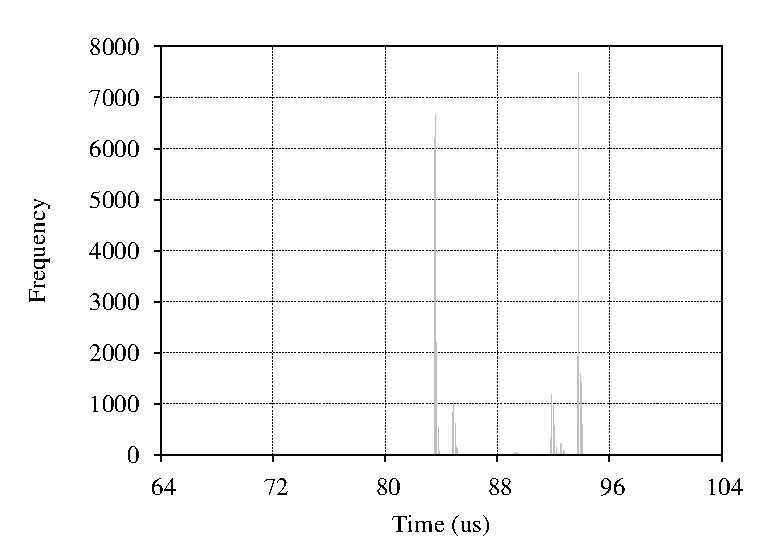
\includegraphics[width=.315\textwidth]{chapter6/figures/rt1}
    \label{fig:rtdelayone}
}
\subfigure[System with four RT-VCPUs.]{
    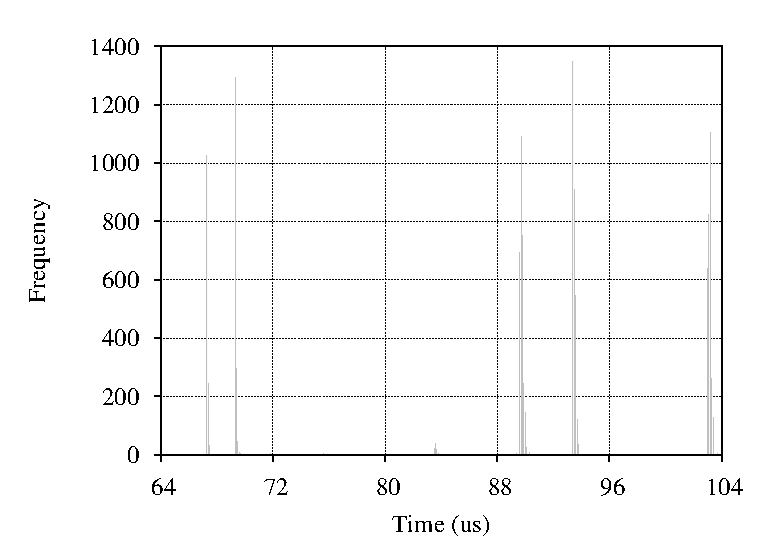
\includegraphics[width=.315\textwidth]{chapter6/figures/rt4}
    \label{fig:rtdelayfour}
}
\subfigure[System with eight RT-VCPUs.]{
    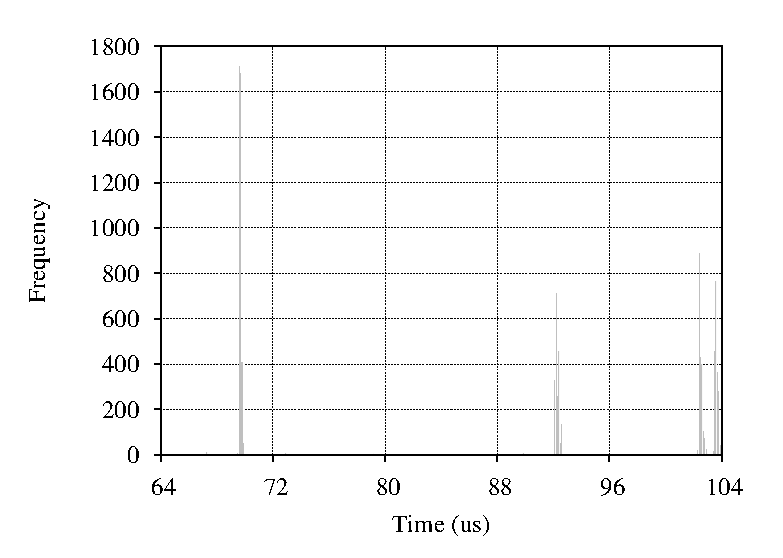
\includegraphics[width=.315\textwidth]{chapter6/figures/rt8}
    \label{fig:rtdelayeigth}
}
\captionsetup{justification=centering}
\caption{Histogram of the execution delay for RT-VCPUs in microseconds.}
\label{fig:rtdelay}
\end{figure}


Table \ref{table:rtdelay} shows the average, standard deviation, median and the $95^{th}$ percentile after 10,000 scheduling rounds for each number for RT-VCPUs in microseconds. The corresponding histograms for the execution of the 1, 4 and 8 RT-VCPUs are shown in Figures \ref{fig:rtdelayone}, \ref{fig:rtdelayfour} and \ref{fig:rtdelayeigth} The average time expended to schedule a RT-VCPU is less than 100 microseconds. When compared to a scheduler quantum of 30ms this represents only 0.003\% of the quantum. However, the standard deviation and the $95^{th}$ percentile increases with a higher number of RT-VCPUs. This is caused by the EDF algorithm implementation that has a complexity of $O(n)$. Despite the increase in the response time to represent only a few microseconds, this can be minimized with a predicable EDF implementation, like proposed by \cite{jagbeer2011}.



\subsection{Interrupt Handling Interference on RT-VCPUs}
\label{subsection:int_rtvcpus}

A sequence of four experiments were performed to show how the Hellfire Hypervisor can be configured to support real-time services while minimizing the interrupt delivery delay on BE-VCPUs. Additionally, these tests determined how RT-VCPUs are influenced by external system interrupts.  For this, the extended real-time services and fast interrupt delivery capabilities were combined in the same virtualized system. The system configuration for this experiment consisted of a Linux guest, a HellfireOS guest and a RT-VM. The Linux guest was responsible for network communication with external devices because it was configured with TCP/IP support and the Ethernet device was directly mapped to it. The HellfireOS was responsible for managing the real-time services (start and stop). The RT-VM implemented a real-time service to perform the ADPCM algorithm (see Subsection \ref{section:hellfireOverhead}). When the algorithm is encoding or decoding for sound reproduction purposes, it must keep a constant bit rate to avoid sound glitches. Thus, the hypervisor must guarantee that concurrent events will not affect the ADPCM execution. 


\begin{figure}[!hbtp]
	\centering
	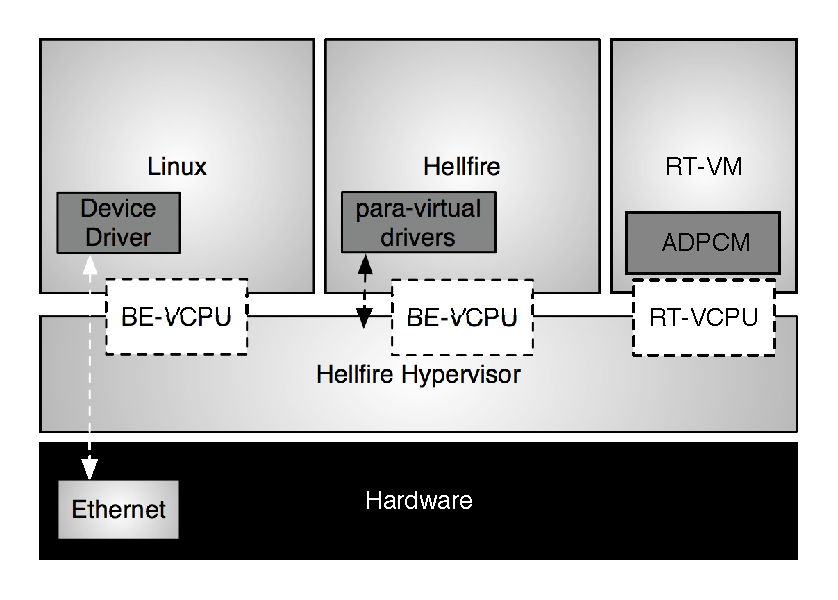
\includegraphics[width=0.40\textwidth]{chapter6/figures/rtsystem}
	\caption{System configuration for the ADPCM execution.}
	\label{fig:rtsystem}
\end{figure}


On the RT-VM, the ADPCM algorithm was mapped to a RT-VCPU that is scheduled by the EDF algorithm, as explained in Subsection \ref{subsection:best-effort-edf}. The real-time parameters of the RT-VCPU were: deadline 10, period 10, and capacity 1. Thus,  a tenth of the processor's time is reserved for the RT-VCPU. The remaining time is available to the BE-VCPUs responsible for executing the Linux and HellfireOS guests. The final system configuration consisted of two BE-VCPUs and 1 RT-VCPU. Figure \ref{fig:rtsystem} shows this arrangement. Similar to the experiment shown in Section \ref{section6:interruption-delay}, the ping tool was used to generate echo request messages from a host computer to the SEAD-3 board at a rate of 20Hz.

\begin{table}[!hbtp]
\centering
\caption{Average ($\overline{x}$), standard deviation ($s$), median ($m$), $95^{th}$ percentile ($p^{th}$), worst execution case (WEC) and best execution case (BEC) to ADPCM encoding and decoding and the RTT of the messages for different system configurations in milliseconds.}
\label{table:rtsystem}
\begin{tabular}{lllllllll}
\hline \hline \\
\textbf{\#}                 & \textbf{System Conf.}                                   & \textbf{Test}     & \textbf{$\overline{x}$} & \textbf{$s$} & \textbf{$m$} & \textbf{$p^{th}$} & \textbf{WEC} & \textbf{BEC} \\ \\ \hline
\multirow{3}{*}{\textbf{1}} & \multirow{3}{*}{\textbf{Execution time}} & \textbf{Encoding} & 1366.58    & 134.21     & 1487       & 1487       & 1487        & 1217        \\
                            &                                                     & \textbf{Decoding} & 1068.94    & 133.1      & 1187       & 1188       & 1188        & 917  \\       
                            &                                                     & \textbf{RTT}      &  1.073 &   0.107 &    1.05 &   1.24     & 3.25   & 0.99                       \\  \hline            
\multirow{3}{*}{\textbf{2}} & \multirow{3}{*}{\textbf{Non policy}}                & \textbf{Encoding} & 1375.27    & 133.16     & 1487       & 1488       & 1488        & 1216        \\
                            &                                                     & \textbf{Decoding} & 1082.17    & 148.63     & 1188       & 1188       & 1189        & 917         \\
                            &                                                     & \textbf{RTT} & 13.37      & 15.1       & 5.78       & 45.5       & 66.6        & 0.78        \\ \hline
\multirow{3}{*}{\textbf{3}} & \multirow{3}{*}{\textbf{Fast policy - non-RT}}        & \textbf{Encoding} & 2004.25    & 546.48     & 2082       & 2705       & 2997        & 1217        \\
                            &                                                     & \textbf{Decoding} & 1505.45    & 497.15     & 1211       & 2390.1     & 2677        & 917         \\
                            &                                                     & \textbf{RTT} & 2.077      & 4.8        & 1.45       & 1.74       & 63.6        & 1.07        \\ \hline
\multirow{3}{*}{\textbf{4}} & \multirow{3}{*}{\textbf{Fast Policy - RT}}            & \textbf{Encoding} & 1378.48    & 132.55     & 1487       & 1488       & 1490        & 1217        \\
                            &                                                     & \textbf{Decoding} & 1081.0     & 132.12     & 1188       & 1188       & 1188        & 917         \\
                            &                                                     & \textbf{RTT} & 3.60       & 7.26       & 1.48       & 20.81      & 65.8        & 1.05        \\ \hline
\end{tabular}
\end{table}

\begin{figure}[!hbtp]
	\centering
	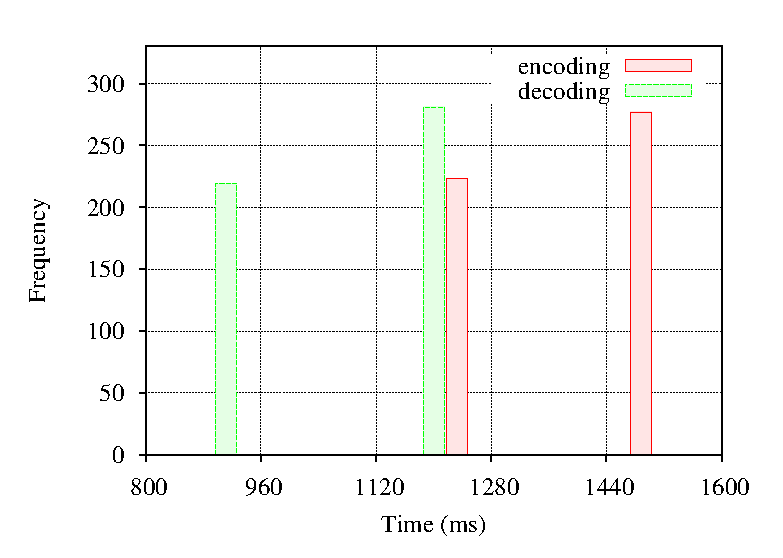
\includegraphics[width=0.50\textwidth]{chapter6/figures/non_int}
	\caption{Histogram of encoding and decoding execution time for the ADPCM algorithm without external interferences.}
	\label{fig:nonint}
\end{figure}


\textbf{Experiment 1.} The first experiment determined how much time the ADPCM algorithm takes to encode and decode a data array. The algorithm was performed during 1,000 encoding and decoding cycles and the time of each execution was recorded. Table \ref{table:rtsystem} shows the numeric results for this experiment in line 1. Additionally, it was plotted in the histogram shown in Figure \ref{fig:nonint}. During this experiment, the RT-VCPU was performed alone and all external interrupts were masked. Thus, obtaining the execution time without the influence of other VCPUs or interrupts. The worst case execution time for encoding was 1,487 ms and 1,217 ms for decoding. Moreover, line one of Table \ref{table:rtsystem} shows the RTT of the messages for native Linux execution for comparison purposes with the upcoming experiments. 

\textbf{Experiment 2.} The second experiment showed the behavior of the ADPCM execution time and the RTT of the messages when the fast delivery policy was not used. This is the simplest configuration, where all interrupts are postponed to the next execution of the target VCPU. This scheme guarantees a temporal isolation to the RT-VCPU since interrupts to other VMs do not preempt its execution. The histogram for 1,000 encoding and decoding cycles is shown in Figure \ref{fig:hist-non-fast}. Additionally, line 2 of the Table \ref{table:rtsystem} shows the numeric results. It confirms that the ADPCM's execution time was not affected by the external interrupts since it is similar to the histogram in Figure \ref{fig:nonint}. However, this scheme had an undesired effect over the RTT of the messages: the average response time increased substantially. Figure \ref{fig:hist-ping-non-fast} is a histogram for 10,000 messages recorded during the experiment. The histogram for the RTT of the messages for native Linux execution can be seen in Figure \ref{fig:native}.

\begin{figure}[!hbtp]
\centering
\subfigure[Histogram of encoding and decoding time for the ADPCM algorithm.]{
    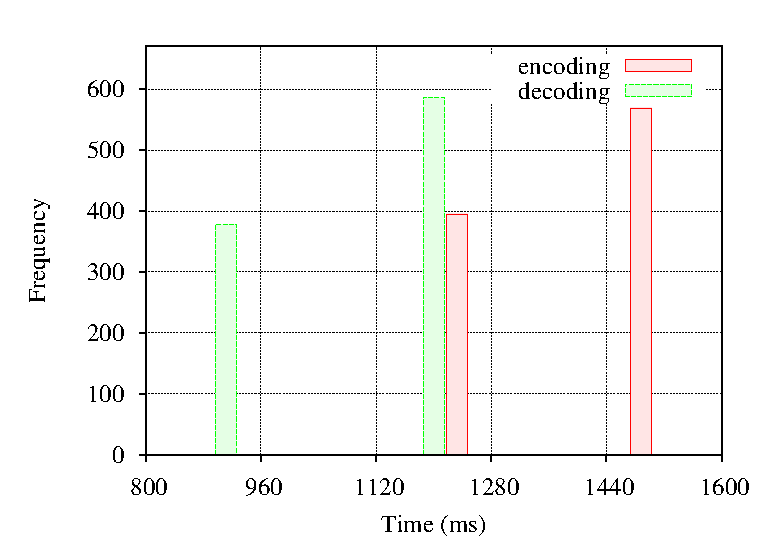
\includegraphics[width=.48\textwidth]{chapter6/figures/20hz_int}
    \label{fig:hist-non-fast}
}
\subfigure[Histogram for RTT of the messages.]{
    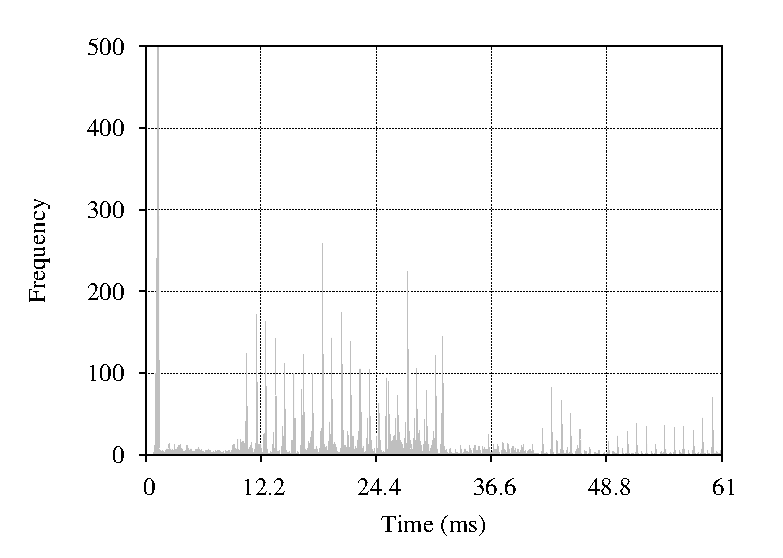
\includegraphics[width=.48\textwidth]{chapter6/figures/ping-non-fast-int}
    \label{fig:hist-ping-non-fast}
}

\captionsetup{justification=centering}
\caption{System response time without the fast interrupt deliver policy and a preemptable RT-VM.}
\label{fig:histogram_nonpremp_nonfast}
\end{figure}

\textbf{Experiment 3.} The third experiment tried to minimize the RTT of the ICMP messages applying the fast interrupt delivery policy. However, the RT-VM was kept as preemptable for an evaluation of how system interrupts can intervene on the RT-VCPU's execution. Thus, both the RT-VCPU and the HellfireOS could be preempted for interrupts targeting the Linux guest. Similar to the previous experiments, 1,000 ADPCM encoding and decoding cycles and 10,000 messages RTT were recorded. Figure \ref{fig:histogram_premp_fast} shows the resulting histograms. The numerical results can be seen in line 3 of Table \ref{table:rtsystem}.

\begin{figure}[!hbtp]
\centering
\subfigure[Histogram of encoding and decoding time for the ADPCM algorithm.]{
    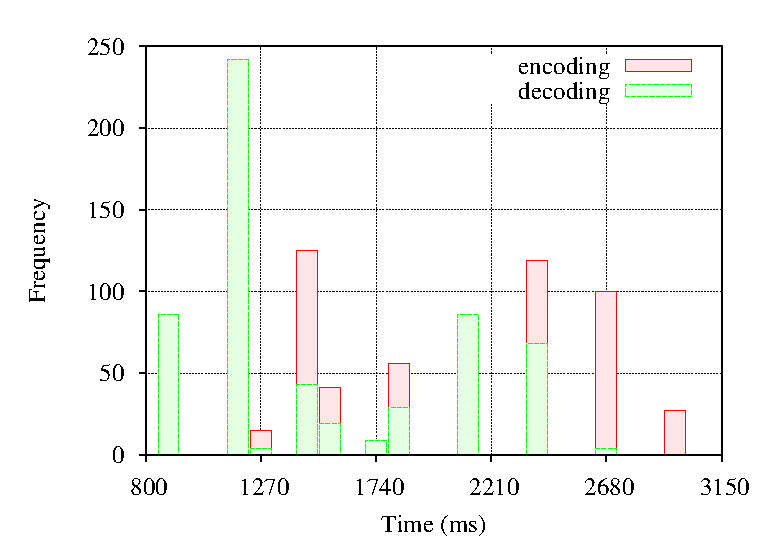
\includegraphics[width=.48\textwidth]{chapter6/figures/nonrt-fast}
    \label{fig:hist-nonrt-fast}
}
\subfigure[Histogram for RTT of the messages.]{
    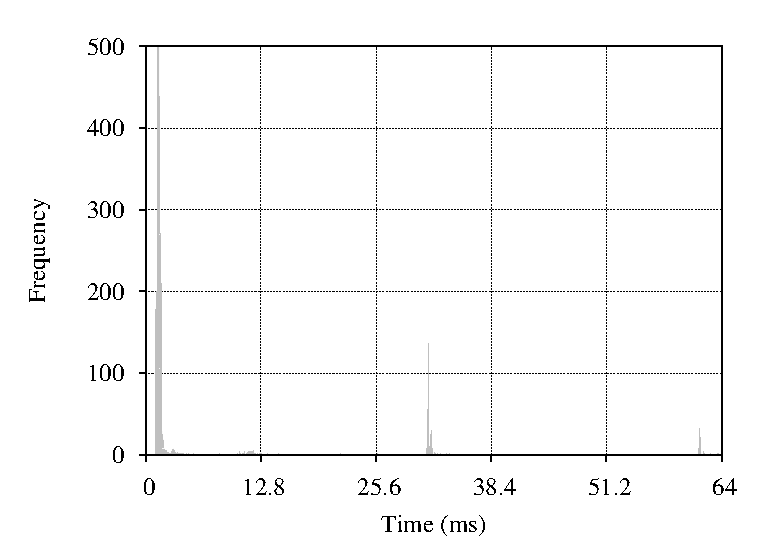
\includegraphics[width=.48\textwidth]{chapter6/figures/ping-nonrt-fast}
    \label{fig:hist-ping-nonrt-fast}
}

\captionsetup{justification=centering}
\caption{System response time with the fast interrupt deliver policy and a preemptable RT-VM.}
\label{fig:histogram_premp_fast}
\end{figure}

Figure \ref{fig:hist-ping-nonrt-fast} and the numerical results show that the RTT of the messages improved significantly. Most of the RTTs were near native execution (see Figure \ref{fig:native}). However, some RTTs suffered a long delay, around 31 ms and 61 ms. This is result of the fast interrupt policy with recycled quantum. The recycled quantum was used to preserve the scheduling time coherency to the EDF algorithm. Despite the reset quantum scheme resulting in an improved interrupt response time, as shown in Section \ref{section6:interruption-delay}, it can not be used in combination with RT-VCPUs. Thus, the long delay is due to the insufficient time remaining in the current quantum. Moreover, the interrupt handling finishes only on the next Linux guest execution. On the other hand, Figure \ref{fig:hist-nonrt-fast} showed that ADPCM execution time was affected, increasing significantly. The numerical results can be seen in line 3 of the Table  \ref{table:rtsystem}.

\textbf{Experiment 4.} The fourth experiment consisted of combining the fast interrupt delivery policy with a non-preemptable RT-VM. This system configuration provides the best temporal isolation for RT-VCPUs while improving the response for external interrupts. This is possible because the fast interrupt delivery policy preempts the VCPUs for faster response time. However, the RT-VM is marked as non-preemptable resulting that its RT-VCPUs cannot be preempted. This guarantees a tenth of the CPU to the  RT-VCPU executing the ADPCM algorithm. 

\begin{figure}[!hbtp]
\centering
\subfigure[Histogram of encoding and decoding time for the ADPCM.]{
    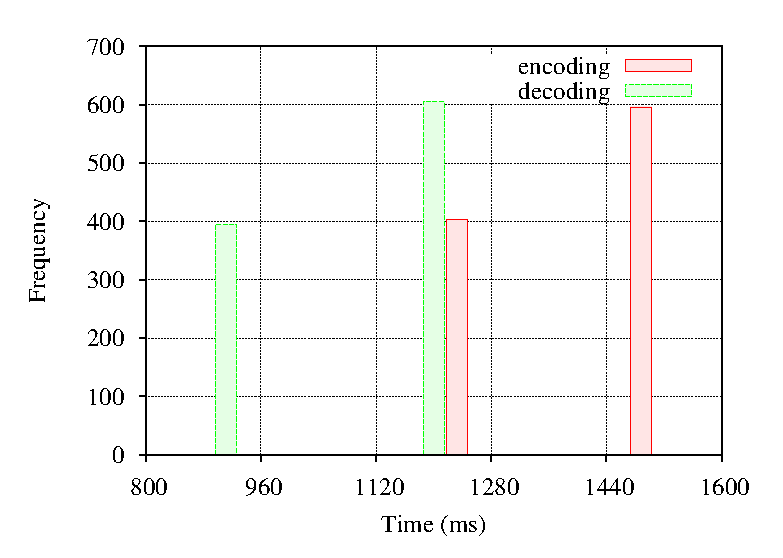
\includegraphics[width=.48\textwidth]{chapter6/figures/rt-fast}
    \label{fig:hist-rt-fast}
}
\subfigure[Histogram for the  RTT of the messages.]{
    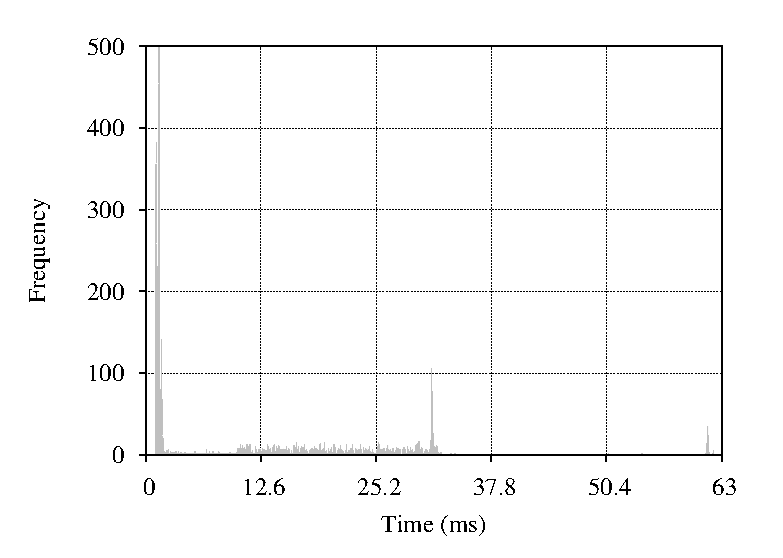
\includegraphics[width=.48\textwidth]{chapter6/figures/ping-rt-fast}
    \label{fig:hist-ping-rt-fast}
}
\captionsetup{justification=centering}
\caption{System response time with the fast interrupt deliver policy and a non-preemptable RT-VM.}
\label{fig:histogram_rt_fast}
\end{figure}

Line 4 of Table \ref{table:rtsystem} shows the numerical results for this experiment. The worst execution case to encoding and decoding the ADPCM algorithm is similar to the execution time presented in line 1 (non external interference). Moreover, the histogram for the execution time shown in Figure \ref{fig:hist-rt-fast} is similar to the histogram in Figure \ref{fig:nonint}. This shows the effectiveness of the temporal isolation provided by the hypervisor. In addition, the RTT of the messages improved significantly. The histogram in Figure \ref{fig:hist-ping-rt-fast} shows that some RTTs are spread between 0.7 and 31ms. This is caused by the RT-VCPU in the RT-VM. The ICMP messages arrived during its execution are delayed until the end of the quantum. The peak near 31ms and 61ms is due to the recycling quantum scheme, as explained before. 


\section{Final Considerations}
\label{section6:finalcons}

This chapter studied the effectiveness of the hypervisor implementation. A sequence of experiments was performed in the SEAD-3 development board to evaluate different aspects of the hypervisor. One important aspect discussed was the footprint. A direct comparison with all other hypervisors studied is not possible because some of them do not mention their footprint. However, the Hellfire Hypervisor's footprint is acceptable for IoT devices, and is similar to the smallest hypervisors with a known  footprint. The overhead impact on Linux was determined using benchmarks for virtualized and non-virtualized executions. User-land applications suffered lower impact than applications that use syscalls intensively. However, the overall overhead is small and comparable to other hypervisors. Moreover, the hypervisors present a low overhead for directly mapped devices. The fast interrupt delivery mechanism was evaluated showing the effectiveness of this policy. This experiment showed that the hardware-assisted virtualization can be used to improve responsiveness while keeping the simplicity of the implementation. The inter-VM communication mechanism presented a considerable overhead caused by the data copies between the VMs and the hypervisor. However, the usage of the hypervisor as a communication arbiter improves the security. Also, shared memory can be used to implement inter-VM communication with lower overhead. Finally, the real-time services were evaluated. The average time expended for RT-VCPU scheduling is lower than 100us in a system with 8 VCPUs. The temporal isolation was tested showing that the fast interrupt policy with non-preemptable RT-VMs is an effective method to combine real-time tasks and fast interrupt handling. The overall results are promising and prove that the hypervisor implementation is efficient in performance and responsiveness. 

